% MTL730 -- Post Mid-Semester Lectures
\documentclass[12pt]{article}

\usepackage[a4paper,margin=0.75in]{geometry}
\usepackage{amsmath,amssymb,amsthm,mathtools}
\usepackage{enumitem}
\usepackage{graphicx}
\usepackage{array}
\usepackage{float}
\usepackage{setspace}
\usepackage{tikz}
\usepackage{microtype}
\usepackage{hyperref}
\usepackage{tcolorbox}
\tcbuselibrary{skins,breakable}

\newtcolorbox{keybox}[1][]{enhanced, breakable,
    colback=white, colframe=black, coltitle=black, colbacktitle=white, titlerule=0.4pt,
    boxrule=0.7pt, arc=2pt, left=7pt, right=7pt, top=2pt, bottom=4pt,
    before skip=12pt, after skip=12pt, fonttitle=\bfseries, #1}

\hypersetup{
    colorlinks=true,
    linkcolor=blue,
    urlcolor=blue,
    citecolor=blue
}

\setstretch{1.17}
\setlength{\parskip}{0.55em plus 0.15em minus 0.08em}
\setlength{\parindent}{1.2em}
\setlength{\abovedisplayskip}{12pt plus 4pt minus 6pt}
\setlength{\belowdisplayskip}{12pt plus 4pt minus 6pt}
\setlength{\abovedisplayshortskip}{8pt plus 3pt}
\setlength{\belowdisplayshortskip}{8pt plus 3pt}
\setlength{\floatsep}{14pt plus 4pt minus 4pt}
\setlength{\textfloatsep}{16pt plus 4pt minus 4pt}
\setlength{\intextsep}{14pt plus 4pt minus 3pt}

\setlist{topsep=0.55em, partopsep=0.2em, itemsep=0.38em, parsep=0.12em}

\makeatletter
\renewcommand{\section}{\@startsection{section}{1}{\z@}%
    {-4.4ex \@plus -1.2ex \@minus -.2ex}%
    {2.6ex \@plus .35ex}%
    {\normalfont\Large\bfseries}}
\renewcommand{\subsection}{\@startsection{subsection}{2}{\z@}%
    {-3.5ex \@plus -1ex \@minus -.2ex}%
    {1.8ex \@plus .25ex}%
    {\normalfont\large\bfseries}}
\def\thm@space@setup{%
    \thm@preskip=0.95em plus 0.35em minus 0.2em
    \thm@postskip=0.95em plus 0.35em minus 0.2em
}
\makeatother

\setcounter{tocdepth}{2}

\newcommand{\lectureheading}[1]{%
    \clearpage
    \phantomsection
    \addcontentsline{toc}{part}{#1}%
    \section*{#1}
    \vspace{0.35em}%
}

\newtheorem{theorem}{Theorem}[section]
\newtheorem{lemma}[theorem]{Lemma}
\newtheorem{proposition}[theorem]{Proposition}
\newtheorem{corollary}[theorem]{Corollary}
\newtheorem{definition}[theorem]{Definition}
\newtheorem{example}[theorem]{Example}
\newtheorem{claim}[theorem]{Claim}
\theoremstyle{remark}
\newtheorem*{remark}{Remark}

\makeatletter
\def\thm@space@setup{%
    \thm@preskip=0.95em plus 0.35em minus 0.2em
    \thm@postskip=0.95em plus 0.35em minus 0.2em
}
\makeatother

\DeclareMathOperator{\gcdop}{gcd}
\DeclareMathOperator{\ord}{ord}
\DeclareMathOperator{\ind}{ind}
\newcommand{\Z}{\mathbb Z}
\newcommand{\N}{\mathbb N}
\newcommand{\R}{\mathbb R}
\newcommand{\Fp}{\mathbb F_p}
\newcommand{\units}[1]{\left(\mathbb Z/#1\mathbb Z\right)^\times}

\title{\textbf{MTL730 --- Post Mid-Semester Lectures}\\[2mm]
\large Discrete Logarithms, RSA, Factorization, and Elliptic Curves}
\author{Crafted by Arpit's Milo}
\date{}

\begin{document}
\maketitle
\begingroup
\setlength{\parskip}{0.12em plus 0.05em}
\setstretch{1.08}
\tableofcontents
\endgroup
\newpage

\lectureheading{Lecture 13 (22/09/26)}

% --- page 01 ---

\section{Difficulty of the discrete logarithm}

How difficult is it to solve the discrete logarithm problem?
Recall from Lecture~12 that, for a prime \(p\), a primitive root \(g\) modulo \(p\), and \(h\in\units{p}\), the DLP asks for the integer \(x\) with \(1\le x\le p-1\) and \(g^{x}\equiv h\pmod{p}\), that is \(x=\ind_{g}(h)\). In a general group the same problem is the equation \(g^{x}=h\).

\begin{example}[An additive group]
Recall from Lecture~12 that solving the discrete logarithm can be easy in certain groups.
In the additive group \((\Z/p\Z,+)\), one is given \(g,h\in\Z/p\Z\) with
\(\gcdop(g,p)=1\), and one must find \(x\) such that
\[
    xg \equiv h \pmod{p}.
\]
The solution is
\[
    x \equiv g^{-1}h \pmod{p},
\]
and computing the inverse is easy. The same symbols in the multiplicative group \(\units{p}\) hide an apparently hard search.
\end{example}

% The date (22/09/26) is written on the page at this point.

How long does it take to solve the discrete logarithm problem?

\begin{remark}
Let \(G\) be a group and let \(g\in G\) be an element of order \(N\), so
\(g^N=e\). The equation \(g^x=h\) can be solved in \(O(N)\) steps, by
testing the powers of \(g\) one at a time. This bound is trivial. It is
also exponential in the input length: \(O(N)\) is of size \(e^{\log N}\).
% p.01: the marginal note beside ``Trivial'' is \(e^{\log N}\), i.e. the \(O(N)\) search is exponential in the input length.
\end{remark}

\begin{remark}
Depending on the group \(G\), one can do better. As in the additive example of Lecture~12, the congruence \(xg\equiv h\pmod{n}\) in \((\Z/n\Z,+)\) is ordinary linear arithmetic whenever \(\gcdop(g,n)=1\).
\end{remark}

% ============================================================
\section{Shanks' baby-step giant-step algorithm}
% ============================================================

% FIX p.01: the heading on the page is ``Shank's''.

\begin{keybox}
\begin{theorem}[Shanks]
Let \(G\) be a group, let \(g\in G\) be an element of order \(N\) with
\(N\ge 2\), and let \(h\in\langle g\rangle\). The discrete logarithm
\(g^x=h\) can be solved in \(O(\sqrt{N}\log N)\) steps. In particular
the running time is \(O(N^{1/2+\varepsilon})\) for every \(\varepsilon>0\).
% FIX p.01: under \(O(\sqrt{N}\log N)\) the page first writes \(O(N^{\varepsilon})\) for any \(\varepsilon>0\), strikes it out, and replaces it by \(O(N^{1/2+\varepsilon})\). The struck bound is too small; \(O(\sqrt{N}\log N)=O(N^{1/2+\varepsilon})\) is the right comparison.
\end{theorem}
\end{keybox}

% --- page 02 ---

The algorithm is as follows. Write
\[
    n = \bigl\lfloor\sqrt{N}\bigr\rfloor + 1,
\]
so that \(n>\sqrt{N}\). Form the two lists
\begin{align*}
    \text{List 1}&\colon
        e,\; g,\; g^2,\; \ldots,\; g^{n-1}
        &&\text{(baby steps),}\\[0.3em]
    \text{List 2}&\colon
        h,\; hg^{-n},\; hg^{-2n},\; \ldots,\; hg^{-(n-1)n}
        &&\text{(giant steps).}
\end{align*}
With \(u=g^{-n}\), List~2 is the same as
\[
    h,\; hu,\; hu^2,\; \ldots,\; hu^{n-1}.
\]

\begin{claim}
The two lists have an element in common. If
\[
    g^i = h\cdot g^{-jn},
\]
then \(h=g^{i+jn}\), and the discrete logarithm is
\[
    x = i+jn.
\]
\end{claim}

\begin{proof}
First, every integer \(k\) with \(0\le k\le N\) may be written
\(k=nq+r\) where \(0\le r<n\). The quotient satisfies
\[
    0\le q < n,
\]
because
\[
    q = \frac{k-r}{n} \le \frac{N}{n} < n.
\]
The last inequality holds since \(n>\sqrt{N}\).

Since \(h\in\langle g\rangle\), one has \(h=g^k\) for some
\(0\le k<N\). Write \(k=nq+r\) with \(0\le q,r<n\), as above. Then
\[
    h = g^k = g^{nq+r},
\]
and therefore
\[
    h\cdot g^{-nq} = g^r.
\]
The left-hand side lies in List~2 and the right-hand side lies in
List~1, so the two lists have an element in common. In the notation of
the claim, \(i=r\) and \(j=q\).
\end{proof}

% --- page 03 ---

It remains only to count steps. List~1 is built with \(n\)
multiplications, and List~2 is built with \(n\) multiplications. Sorting
List~1 takes \(O(n\log n)\) steps. Each of the \(n\) elements of List~2
can then be tested for membership in List~1 in \(O(\log n)\) steps.
The total is
\[
    O(n\log n) = O\bigl(\sqrt{N}\log N\bigr).
\]

\begin{example}[Baby-step giant-step modulo \(31\)]
Take \(p=31\) and \(G=\Fp^\times=\units{p}\). The residue \(3\)
is a primitive root, so let \(g=3\). The order of \(g\) is
\(N=p-1=30\), and
\[
    n=\bigl\lfloor\sqrt{30}\bigr\rfloor+1=6.
\]
% FIX p.03: the page writes \(\lfloor\sqrt{31}\rfloor+1=6\). The order is \(N=30\), and \(\lfloor\sqrt{30}\rfloor+1\) is the same integer, so the lists are unchanged.
List~1, the powers \(g^0,\ldots,g^{5}\) modulo \(31\), is
\[
    1,\; 3,\; 9,\; 27,\; 19,\; 26.
\]
Here \(g^n=3^6\equiv 16\pmod{31}\), so \(g^{-n}\equiv 16^{-1}\equiv 2\pmod{31}\).

For \(h=17\), List~2 is
\[
    17,\; 17\cdot 16^{-1},\; 17\cdot 16^{-2},\; \ldots,\; 17\cdot 16^{-5},
\]
which begins
\[
    17,\; 17\cdot 2,\; 17\cdot 4,\; \ldots.
\]
The second entry is \(17\cdot 2=34\equiv 3\pmod{31}\), and \(3=g^1\) lies
in List~1. Thus
\[
    3^1 = 17\cdot 3^{-6},
\]
so \(17=3^7\) and \(x=7\).

For \(h=11\), List~2 is
\[
    11,\; 11\cdot 2,\; 11\cdot 4,\; 11\cdot 8,\; 11\cdot 16,\; 11\cdot 32,
\]
which reduces modulo \(31\) to
\[
    11,\; 22,\; 13,\; 26,\; 21,\; 11.
\]
The entry \(26\) lies in List~1, since \(3^5\equiv 26\pmod{31}\), and
\(26\equiv 11\cdot 8=11\cdot 2^3\pmod{31}\). As \(2\equiv 3^{-6}\), one has
\(2^3\equiv 3^{-18}\), and therefore
\[
    3^5 = 11\cdot 3^{-18}.
\]
Hence \(3^{23}\equiv 11\pmod{31}\), so \(x=23\).
\end{example}

% --- page 04 ---

% ============================================================
\section{The Pohlig--Hellman algorithm}
% ============================================================

% FIX p.06: the page spells the name ``Pohlig--Heuman''.

Recall from Lecture~12 that if the order of \(g\) is smooth, Pohlig--Hellman solves the discrete logarithm efficiently. Given \(g^x=h\), it is enough
to find \(x\pmod{N}\), where \(N\) is the order of \(g\).

\begin{example}[A smooth order: \(p=271\)]
Let \(p=271\), and let \(g=6\), a primitive root modulo \(271\). Then
\[
    p-1 = 270 = 2\cdot 3^3\cdot 5,
\]
so it is enough to solve the discrete logarithm modulo \(2\), modulo
\(27\), and modulo \(5\). Take \(h=145\), and write \(h=g^x\).

Since \(g\) is a primitive root, \(g^{(p-1)/2}\equiv -1\pmod{p}\), and
\[
    h^{(p-1)/2}
    = g^{x(p-1)/2}
    = (-1)^x
    =
    \begin{cases}
        1, & \text{if \(x\) is even},\\
        -1, & \text{if \(x\) is odd}.
    \end{cases}
\]
The same power is the Legendre symbol \(\bigl(\frac{h}{p}\bigr)\).
Compute
\begin{align*}
    \Bigl(\frac{h}{p}\Bigr)
    = \Bigl(\frac{145}{271}\Bigr)
    &= \Bigl(\frac{5}{271}\Bigr)\Bigl(\frac{29}{271}\Bigr)
     = \Bigl(\frac{271}{5}\Bigr)\Bigl(\frac{271}{29}\Bigr)\\
    &= \Bigl(\frac{1}{5}\Bigr)\Bigl(\frac{10}{29}\Bigr)
     = \Bigl(\frac{2}{29}\Bigr)\Bigl(\frac{5}{29}\Bigr)
     = (-1)\cdot\Bigl(\frac{4}{5}\Bigr)
     = -1.
\end{align*}
% The factor \(\bigl(\frac{1}{5}\bigr)\) is crossed out on the page once it is seen to equal \(1\).
% Filled step: \(5\equiv 29\equiv 1\pmod{4}\), so quadratic reciprocity gives the two flips; \(271\equiv 1\pmod{5}\) and \(271\equiv 10\pmod{29}\); \(10=2\cdot 5\); \(\bigl(\frac{2}{29}\bigr)=-1\) because \(29\equiv 5\pmod{8}\); and \(\bigl(\frac{5}{29}\bigr)=\bigl(\frac{29}{5}\bigr)=\bigl(\frac{4}{5}\bigr)=1\).
Thus \(x\) is odd:
\[
    x\equiv 1\pmod{2}.
\]

% --- page 05 ---

Next one finds \(x\pmod{5}\). Compare
\[
    h^{(p-1)/5}
    \qquad\text{with}\qquad
    g^{(p-1)/5},\;
    g^{2(p-1)/5},\;
    g^{3(p-1)/5},\;
    g^{4(p-1)/5},\;
    g^{5(p-1)/5}.
\]
Since \((p-1)/5=54\),
\[
    145^{54}\equiv 1\pmod{p},
\]
and therefore \(x\equiv 0\pmod{5}\).

To see the shape of this congruence, write \(x=5k+m\). Then
\(h=g^x=g^{5k+m}\), so
\[
    h^{(p-1)/5}
    = g^{(5k+m)(p-1)/5}
    = g^{m(p-1)/5},
\]
the term in \(k\) disappearing because \(g^{p-1}\equiv 1\). The value
\(1\) occurs precisely for \(m\equiv 0\pmod{5}\).

Next one calculates \(x\pmod{27}\). Expand
\[
    x = c_0 + c_1\cdot 3 + c_2\cdot 3^2,
    \qquad 0\le c_i\le 2.
\]
Modulo \(p\),
\[
    g^{(p-1)/3}\equiv 242, \qquad
    g^{2(p-1)/3}\equiv 28, \qquad
    h^{(p-1)/3}\equiv 28.
\]
The last two agree, so \(c_0=2\).

To find \(c_1\), write \(h=g^x=g^{c_0+3c_1+3^2 c_2}\). Then
\[
    \frac{h}{g^{c_0}}
    = g^{3c_1+3^2 c_2}
    = g^{3(c_1+3c_2)},
\]
% FIX p.05: the middle exponent is written \(3^2 c_1\). The next expression is \(g^{3(c_1+3c_2)}\), so the factor must be \(c_2\).
and raising to the power \((p-1)/9\) isolates the next digit:
\[
    \Bigl(\frac{h}{g^{c_0}}\Bigr)^{(p-1)/9}
    = g^{c_1(p-1)/3}.
\]
% FIX p.05: the denominator is the digit \(9\). The loop looks like a \(q\), but \(q\) is not defined here, and the identity needs \((p-1)/9\): the left side is \(g^{3(c_1+3c_2)}\), so the exponent \((p-1)/9\) produces \(g^{c_1(p-1)/3}\).
The notes say to continue from here. Carrying out that arithmetic:
\(g^{c_0}=6^2\equiv 36\), and
\[
    h\cdot g^{-c_0}\equiv 132\pmod{271},
    \qquad
    132^{(p-1)/9}=132^{30}\equiv 28
    \equiv g^{2(p-1)/3}\pmod{271},
\]
so \(c_1=2\). One further step, with \(c_0+3c_1=8\), gives
\[
    h\cdot g^{-8}\equiv 3\pmod{271},
    \qquad
    3^{(p-1)/27}=3^{10}\equiv 242
    \equiv g^{(p-1)/3}\pmod{271},
\]
so \(c_2=1\). Therefore
\[
    x\pmod{27}
    = c_0+3c_1+9c_2
    = 2+6+9
    = 17.
\]
% Filled step: the page writes ``\(\ldots\) continue'' and then the answer \(c_1=2\), \(c_2=1\).
\end{example}

% --- page 06 ---

The three congruences are
\[
    \left.
    \begin{aligned}
        x&\equiv 1 \pmod{2}\\
        x&\equiv 0 \pmod{5}\\
        x&\equiv 17\pmod{27}
    \end{aligned}
    \right\}
    \qquad
    x\equiv 125\pmod{270}.
\]
% Filled step: the page records the result of the Chinese remainder theorem and not the arithmetic. From \(x=27t+17\equiv 0\pmod{5}\) one gets \(2t\equiv 3\pmod{5}\), so \(t\equiv 4\pmod{5}\) and \(x\equiv 125\pmod{270}\). The class \(125\) is already odd, so the condition modulo \(2\) holds as well. And \(6^{125}\equiv 145\pmod{271}\).

\subsection{Primes for which the algorithm does not help}

There is a way out of the improvement above. Let \(p\) be an odd prime, so
that \(p-1\) is even, and suppose that \((p-1)/2\) itself is prime. Set
\[
    q=\frac{p-1}{2},
\]
so that \(p=2q+1\). Baby-step giant-step on the whole group, and on the
subgroup of order \(q\), then cost about \(\sqrt{p}\) and \(\sqrt{q}\)
respectively, and
\[
    \sqrt{p}=\sqrt{2q+1}\approx\sqrt{2q}=\sqrt{2}\,\sqrt{q}.
\]
The two running times are of the same size, so factoring \(p-1=2q\) does
not improve on a direct attack.

\begin{definition}[Sophie Germain prime]
A \emph{Sophie Germain prime} is a prime \(p\) such that \(2p+1\) is also
prime.
\end{definition}
In the notation above, \(q\) is a Sophie Germain prime and \(p=2q+1\) is
prime.

\subsection{The general statement}

\begin{keybox}
\begin{theorem}[Pohlig--Hellman]
Let \(G\) be a group, and suppose that whenever \(g\in G\) has order
\(p^e\) one can solve the discrete logarithm in the subgroup
\(H=\langle g\rangle\) in \(S(p^e)\) steps.
% FIX p.06: the page writes the order as \(p^2\), while the cost on the next line is \(S(p^e)\) and the sum below runs over \(p_i^{e_i}\). The statement is for a general prime power.
Let \(\hat g\in G\) be an
element of order
\[
    N = p_1^{e_1}\cdots p_t^{e_t}.
\]
Then the discrete logarithm in \(\langle\hat g\rangle\) can be solved in
\[
    \sum_{i=1}^{t} S(p_i^{e_i}) + (\log N)^{*}
\]
steps.
% p.06: the second term is \((\log N)^{*}\) on the page. Page~10 identifies it as the Chinese-remainder cost \(O(\log N)\).
\end{theorem}
\end{keybox}

By comparison, baby-step giant-step on a group of order \(N\) costs
\(\sqrt{N}\log N\) steps.

% --- page 07 ---

As a rough comparison, take \(t=2\) with \(p_1\approx p_2\) and
\(e_1=e_2\). Writing \(p\) and \(e\) for those common values, and using
baby-step giant-step as the prime-power routine, so that
\(S(p^e)\) contributes a factor \(p^{e/2}\cdot e\log p\), one gets
\begin{align*}
    S(p_1^{e_1})+S(p_2^{e_2})+(\log N)^{*}
    &= p_1^{e_1/2}\cdot e_1\log p_1
       + p_2^{e_2/2}\cdot e_2\log p_2
       + (\log N)^{*}\\
    &\approx 2\,p^{e/2}\,(\log N)^{*}.
\end{align*}
For \(N\) of size \(p^{2e}\) the direct baby-step giant-step bound
\(\sqrt{N}\log N\) is about \(p^{e}\log N\), larger by a factor about
\(p^{e/2}\).

The algorithm producing the \(y_i\) in the theorem is the following.
The input is \(\hat g^{x}=h\).
\begin{enumerate}[leftmargin=1.6em]
    \item For each \(i\), set
    \[
        g_i = \hat g^{\,N/p_i^{e_i}}
        \qquad\text{and}\qquad
        h_i = h^{\,N/p_i^{e_i}}.
    \]
    The element \(g_i\) has order \(p_i^{e_i}\). Solve the discrete
    logarithm \(g_i^{y_i}=h_i\), and let \(y_i\) be the solution.
    \item Solve the system
    \[
        \begin{cases}
            x\equiv y_1\pmod{p_1^{e_1}},\\
            \qquad\vdots\\
            x\equiv y_t\pmod{p_t^{e_t}}
        \end{cases}
    \]
    by the Chinese remainder theorem. The solution satisfies
    \(\hat g^{x}=h\).
\end{enumerate}

\lectureheading{Lecture 14 (23/09/26)}

% --- page 08 ---

Baby-step giant-step applies to an element \(g\) of order \(N\): the
discrete logarithm in \(\langle g\rangle\), namely \(g^x=h\), can be
solved in \(O(\sqrt{N}\log N)\) steps. For a typical example take
\(G=\units{p}\) with \(p-1\) even, and suppose
\[
    q=\frac{p-1}{2}
\]
is also prime. As on the previous page, Pohlig--Hellman then gives no
substantial saving.

The Pohlig--Hellman theorem is recorded again, together with the
algorithm.

\begin{theorem}
Let \(G\) be a group. Suppose that for any element \(g\) of order
\(p^e\), with \(p\) prime and \(e\ge 1\), the discrete logarithm in
\(\langle g\rangle\) can be solved in \(S(p^e)\) steps. Let \(\hat g\)
be an element whose order is \(p_1^{e_1}\cdots p_t^{e_t}\). Then the
discrete logarithm in \(\langle\hat g\rangle\) can be solved in
\[
    \sum_{i=1}^{t} S(p_i^{e_i}) + (\log N)^{*}
\]
steps, by the following algorithm. Here \(N\) is the order of \(\hat g\).
\end{theorem}

% A line struck through before step~(1) is illegible; it appears to begin ``if \(N\neq p_1\), \(p_1\neq p_2\)''.
% UNCLEAR p.08: struck-out false start immediately before the algorithm.

Let \(\hat g^{x}=h\).
\begin{enumerate}[leftmargin=1.6em]
    \item Let
    \[
        g_i=\hat g^{\,N/p_i^{e_i}},
        \qquad
        h_i=h^{\,N/p_i^{e_i}},
    \]
    and let \(y_i\) be the solution of the discrete logarithm
    \(g_i^{y}=h_i\).
    \item Solve
    \[
        \begin{cases}
            x\equiv y_1\pmod{p_1^{e_1}},\\
            \qquad\vdots\\
            x\equiv y_t\pmod{p_t^{e_t}}
        \end{cases}
    \]
    by the Chinese remainder theorem. The solution satisfies
    \(\hat g^{x}=h\).
\end{enumerate}

% --- page 09 ---

\begin{proof}
The element \(g_i\) has order \(p_i^{e_i}\). If \(\hat g^{x}=h\), then
\(g_i^{x}=h_i=g_i^{y_i}\), so the true discrete logarithm satisfies
\[
    x = y_i + p_i^{e_i}\,k
\]
for some integer \(k\), for each \(i\). Conversely, any integer \(x\) of
this form for every \(i\) is a discrete logarithm, by the calculation
that follows. Substituting the shape of \(x\),
\begin{align*}
    \bigl(\hat g^{x}\bigr)^{N/p_i^{e_i}}
    &= \hat g^{\,(y_i+p_i^{e_i}k)\,N/p_i^{e_i}}
     = \hat g^{\,y_i\,N/p_i^{e_i}}
       \cdot\bigl(\hat g^{N}\bigr)^{k}
     = \hat g^{\,y_i\,N/p_i^{e_i}}\\
    &= g_i^{y_i}
     = h_i
     = h^{\,N/p_i^{e_i}}.
\end{align*}
% p.09: an attempt to conclude \(\hat g^{x}=h\) already at this line is crossed out.
The identity
\[
    \bigl(\hat g^{x}\bigr)^{N/p_i^{e_i}} = h^{\,N/p_i^{e_i}}
\]
therefore holds for every \(i\) with \(1\le i\le t\).

The integers \(N/p_1^{e_1},\ldots,N/p_t^{e_t}\) have gcd \(1\), since
each prime \(p_i\) fails to divide \(N/p_i^{e_i}\) and these are all the
prime factors of \(N\). Hence there exist integers \(c_1,\ldots,c_t\)
such that
\[
    c_1\frac{N}{p_1^{e_1}} + \cdots + c_t\frac{N}{p_t^{e_t}} = 1.
\]
Raising the identity above to the power \(c_i\) gives
\[
    \bigl(\hat g^{x}\bigr)^{c_i N/p_i^{e_i}}
    = h^{\,c_i N/p_i^{e_i}}
\]
for each \(i\). Multiplying these \(t\) equations together, the exponent
on each side is \(\sum c_i N/p_i^{e_i}=1\), and one obtains
\(\hat g^{x}=h\).
\end{proof}

The number of steps splits in the same way as the algorithm.
\begin{itemize}[leftmargin=1.4em]
    \item Step~1, accounting for each \(i\) with \(1\le i\le t\), takes
    \[
        \sum_{i=1}^{t} S(p_i^{e_i})
    \]
    steps.
    \item Step~2 solves a system of linear congruences by the Chinese
    remainder theorem.
\end{itemize}

% --- page 10 ---

For the second step, recall the explicit solution of a Chinese remainder
system. If \(x\equiv b_i\pmod{m_i}\) for \(1\le i\le t\), with the
\(m_i\) pairwise coprime, set \(M=m_1\cdots m_t\) and \(M_i=M/m_i\). Then
\(\gcdop(m_i,M_i)=1\), so there are integers \(N_i\) and \(n_i\) with
\[
    M_i N_i + m_i n_i = 1,
\]
and in particular \(M_i N_i \equiv 1\pmod{m_i}\).
% FIX p.10: the line is \(M_i N_i+m_i n_i=1\), not \(M_i N_i+m_i=1\). The coefficient \(n_i\) is the second Bézout coefficient; only \(N_i\) is used in the sum below.
The integer
\[
    x = \sum_{i=1}^{t} b_i M_i N_i
\]
is a solution. This arithmetic takes \(O(\log N)\) steps, where \(N\) is
the product of the moduli. In the Pohlig--Hellman system one has
\(m_i=p_i^{e_i}\), \(b_i=y_i\), and \(M=N\), so step~2 requires
\(O(\log N)\) steps. This is the term written \((\log N)^{*}\) above.

The prime-power cost \(S(p_i^{e_i})\) will now be reduced to the
prime-order cost \(S(p_i)\):
\[
    S(p_i^{e_i}) = e_i\, S(p_i).
\]

\begin{theorem}[Reduction to prime order]
Let \(G\) be a group and let \(p\) be a prime. Suppose \(g\in G\)
satisfies \(\ord(g)=p\), and that for every such element the discrete
logarithm in \(\langle g\rangle\) can be solved in \(S(p)\) steps. Then
for \(\hat g\in G\) with \(\ord(\hat g)=p^e\) and some \(e\ge 1\), the
discrete logarithm \(\hat g^{x}=h\) in \(\langle\hat g\rangle\) can be
solved in \(O\bigl(e\,S(p)\bigr)\) steps.
\end{theorem}

\begingroup\samepage
Applied to the previous theorem, the discrete logarithm for an element
of order \(N=\prod_i p_i^{e_i}\) can therefore be solved in
\[
    \sum_{i} e_i\, S(p_i) + O(\log N)
\]
steps.
\endgroup

\begin{proof}
One wants to solve \(\hat g^{x}=h\). The unknown may be taken in the
range \(0\le x\le p^e-1\).
% The page writes ``expect \(0\le x<p^e\)'' and, beneath it, ``\(\le p^e-1\)''.
Expand \(x\) in base \(p\),
\[
    x = x_0 + x_1 p + x_2 p^2 + \cdots + x_{e-1}p^{e-1},
    \qquad 0\le x_i<p.
\]
% --- page 11 ---
The digits \(x_i\) are what one has to find. The element
\(\hat g^{\,p^{e-1}}\) has order \(p\).

For the first digit, 
\[
    h^{p^{e-1}}
    = \bigl(\hat g^{x}\bigr)^{p^{e-1}}
    = \hat g^{\,x_0\,p^{e-1}}
    = \bigl(\hat g^{\,p^{e-1}}\bigr)^{x_0},
\]
since every term \(x_j p^j\) with \(j\ge 1\) contributes a multiple of
\(p^e\) to the exponent. Set
\[
    h' = h^{p^{e-1}},
    \qquad
    g' = \hat g^{\,p^{e-1}},
\]
both of which are determined by the input, and \(g'\) has order \(p\).
The displayed equation is \(h'=(g')^{x_0}\), a discrete logarithm for an
element of order \(p\). It is solved in \(S(p)\) steps and returns
\(x_0\). Equivalently, the discrete logarithm in the subgroup
\(\langle\hat g^{\,p^{e-1}}\rangle\) is solved in time \(S(p)\).

For the next digit,
\begin{align*}
    h^{p^{e-2}}
    = \bigl(\hat g^{x}\bigr)^{p^{e-2}}
    &= \hat g^{\,x_0\,p^{e-2}+x_1\,p^{e-1}},\\[0.3em]
    \frac{h^{p^{e-2}}}{\hat g^{\,x_0\,p^{e-2}}}
    &= \bigl(\hat g^{\,p^{e-1}}\bigr)^{x_1}.
\end{align*}
The left-hand side is known once \(x_0\) is known, and the base on the
right has order \(p\). This discrete logarithm is solved in \(S(p)\)
steps and returns \(x_1\).

Continuing in the same way produces every digit \(x_i\). At stage \(i\)
one solves
\[
    \Bigl(
        h\,\hat g^{-(x_0+x_1 p+\cdots+x_{i-1}p^{i-1})}
    \Bigr)^{p^{e-(i+1)}}
    =
    \bigl(\hat g^{\,p^{e-1}}\bigr)^{x_i}
\]
in the subgroup of order \(p\). There are \(e\) digits, so the total
number of steps is \(e\times S(p)\). This completes the proof.
\end{proof}

% --- page 12 ---

\subsection{Comparison of the algorithms}

Baby-step giant-step applies in every case. It is an exponential-time
algorithm. Pohlig--Hellman is useful in some special cases, but it does
not improve the algorithm substantially in many cases, the safeprime
situation above being the typical example.

Index calculus is a subexponential algorithm, of shape
\(e^{\sqrt{\log N}}\), and will be discussed later.
% FIX p.12: the parenthetical is \(e^{\sqrt{\log N}}\), confirmed on the page. The usual index-calculus bound also has a \(\log\log N\) under the square root; the notes omit it. The written shape is still subexponential.

% ============================================================
\section{The RSA cryptosystem}
% ============================================================

The cryptosystem is due to R.~Rivest, A.~Shamir, and L.~Adleman.

\subsection{Factorization of integers}
The main principle is that the public modulus is a product
\[
    N=pq
\]
of two large primes.

\begin{theorem}[Bertrand's postulate]
Between \(n\) and \(2n\) there is a prime, for every integer \(n\ge 2\).
\end{theorem}

If \(p\) and \(q\) are distinct primes, then
\[
    \varphi(pq)=(p-1)(q-1).
\]
Euler's theorem gives: if \(\gcdop(a,pq)=1\), then
\[
    a^{(p-1)(q-1)}\equiv 1\pmod{pq}.
\]
Is this exponent optimal?

For the special case \(p=2\), and \(q\) an odd prime,
% FIX p.12: the page writes \(\varphi(2q)=q-1\) with no hypothesis on \(q\). This holds when \(q\) is an odd prime.
\[
    \varphi(2q)=q-1.
\]
If \(\gcdop(a,2q)=1\), then
\[
    a^{q-1}\equiv 1\pmod{2q}.
\]
This exponent is optimal.
% UNCLEAR p.12: the page ends with the parenthetical ``(primitive root'', cut off at the margin. Read as a reference to primitive roots modulo \(2q\): the group \(\units{2q}\) is cyclic of order \(q-1\), so the exponent \(q-1\) is sharp.

% CONTINUES: exponent of (Z/pqZ)^x, and whether phi(pq)=(p-1)(q-1) is optimal
% --- page 13 ---

If \(p\) and \(q\) are both odd, one can do better. In that case \(p-1\) and \(q-1\) are both even, so \(g=\gcdop(p-1,q-1)\ge 2\) and the exponent below is at most half of \((p-1)(q-1)\).

\begin{keybox}
\begin{theorem}
Let \(p\) and \(q\) be distinct primes, and set \(g=\gcdop(p-1,q-1)\). Then for every integer \(a\) with \(\gcdop(a,pq)=1\),
\[
    a^{(p-1)(q-1)/g}\equiv 1\pmod{pq}.
\]
\end{theorem}
\end{keybox}

\begin{proof}
The quotient \((q-1)/g\) is an integer, and Fermat's little theorem gives \(a^{p-1}\equiv 1\pmod{p}\), so
\[
    a^{(p-1)(q-1)/g}
    =\bigl(a^{p-1}\bigr)^{(q-1)/g}
    \equiv 1\pmod{p}.
\]
The same argument modulo \(q\) yields
\[
    a^{(q-1)(p-1)/g}\equiv 1\pmod{q}.
\]
Thus \(pq\) divides \(a^{(p-1)(q-1)/g}-1\).
\end{proof}

\begin{example}
Take the modulus \(15=3\cdot 5\). Here \(\gcdop(2,4)=2\) and
\[
    \frac{(3-1)(5-1)}{2}=4,
\]
while \(\varphi(15)=8\). The units modulo \(15\) are \(1,2,4,7,8,11,13,14\), and each has fourth power congruent to \(1\):
\begin{align*}
    1^{4}&\equiv 14^{4}\equiv 1,\\
    2^{4}&\equiv 13^{4}\equiv 1,\\
    4^{4}&\equiv 11^{4}\equiv 1,\\
    7^{2}&\equiv 4,\qquad 7^{4}\equiv 8^{4}\equiv 1,
\end{align*}
all modulo \(15\).
% FIX p.13: the notes write a cramped line ``phi(3 x 5) = 8/2 \neq 4''.
% Restored as phi(15)=8 and (p-1)(q-1)/g = 8/2 = 4. The comparison 8 \neq 4 is the point of the example.
In particular
\[
    \gcdop(2,4)=2\implies \varphi(3\cdot 5)=8\neq 4=\frac{8}{2}.
\]
So the exponent \(4\) already works, and it is strictly smaller than \(\varphi(15)\).
\end{example}

Is the exponent \((p-1)(q-1)/g\) optimal?

% --- page 14 ---

Yes. The identity \(\operatorname{lcm}(x,y)=xy/\gcdop(x,y)\) gives
\[
    \frac{(p-1)(q-1)}{g}
    =\frac{(p-1)(q-1)}{\gcdop(p-1,q-1)}
    =\operatorname{lcm}(p-1,q-1).
\]
By the Chinese Remainder Theorem,
\[
    \Z/pq\Z\cong \Z/p\Z\times\Z/q\Z,
\]
and passing to units,
\[
    \units{pq}\cong \units{p}\times\units{q}.
\]

\begin{figure}[H]
\centering
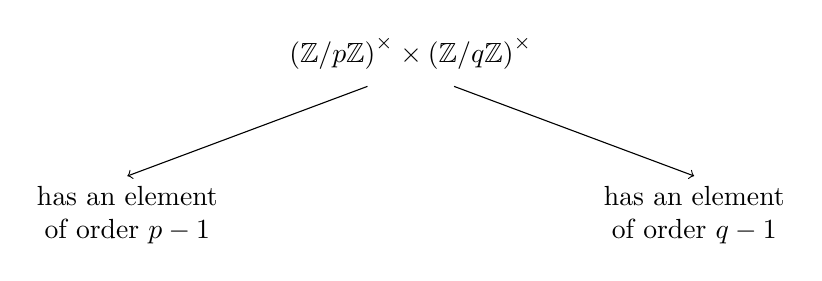
\begin{tikzpicture}
    \node (P) at (0,0.2) {\(\units{p}\times\units{q}\)};
    \node[align=center] (L) at (-3.6,-1.85) {has an element\\ of order \(p-1\)};
    \node[align=center] (R) at ( 3.6,-1.85) {has an element\\ of order \(q-1\)};
    \draw[->] (-0.55,-0.22) -- (L.north);
    \draw[->] ( 0.55,-0.22) -- (R.north);
\end{tikzpicture}
\caption{The two factors of \(\units{pq}\).}
\end{figure}

Each factor is cyclic, so the first has an element of order \(p-1\) and the second an element of order \(q-1\). The corresponding pair in the product then has order \(\operatorname{lcm}(p-1,q-1)\). Hence \(\units{pq}\) has an element of order \(\operatorname{lcm}(p-1,q-1)\), and no smaller positive exponent works for every unit. The exponent in the theorem is optimal.

\begin{remark}
Let \(p\), \(q\), and \(r\) be distinct primes. The largest order of an element of \(\units{pqr}\) is \(\operatorname{lcm}(p-1,q-1,r-1)\). Explicitly, if
\begin{align*}
    a&=\gcdop(p-1,q-1,r-1),&
    b&=\gcdop(p-1,q-1),\\
    c&=\gcdop(q-1,r-1),&
    d&=\gcdop(p-1,r-1),
\end{align*}
then
\[
    \operatorname{lcm}(p-1,q-1,r-1)
    =\frac{(p-1)(q-1)(r-1)\cdot a}{b\cdot c\cdot d}.
\]
\end{remark}

\lectureheading{Lecture 15 (06/10/26)}

Consider the congruence
\[
    x^{e}\equiv c\pmod{N}.
\]
The problem is to find an \(e\)th root of \(c\) modulo \(N\). This is easy when \(N=p\) is prime.

% --- page 15 ---

\begin{proposition}
Let \(p\) be prime and let \(e\ge 1\) satisfy \(\gcdop(e,p-1)=1\). Then the congruence \(x^{e}\equiv c\pmod{p}\) has a unique solution, namely
\[
    x\equiv c^{d}\pmod{p},
\]
where \(ed\equiv 1\pmod{p-1}\).
\end{proposition}

\begin{proof}
If \(c\equiv 0\pmod{p}\), then \(x\equiv 0\pmod{p}\) is a solution. It is the only one: \(p\) divides \(x^{e}\), so \(p\) divides \(x\).

Now assume \(c\not\equiv 0\pmod{p}\), that is \(\gcdop(c,p)=1\). Fermat gives \(c^{p-1}\equiv 1\pmod{p}\). Write \(de=1+k(p-1)\). Then
\begin{align*}
    (c^{d})^{e}
    =c^{de}
    =c^{1+k(p-1)}
    =c\cdot\bigl(c^{p-1}\bigr)^{k}
    \equiv c\cdot 1
    \equiv c\pmod{p}.
\end{align*}
Thus \(x\equiv c^{d}\pmod{p}\) is a solution. If \(x_{1}\) is any other solution, the same congruence \(x_{1}^{p-1}\equiv 1\pmod{p}\) yields
\[
    x_{1}
    \equiv x_{1}^{de}
    =(x_{1}^{e})^{d}
    \equiv c^{d}\pmod{p}.
\]
\end{proof}

\begin{keybox}
\begin{proposition}
Let \(p\) and \(q\) be distinct primes, and let \(e\ge 1\) satisfy \(\gcdop\bigl(e,(p-1)(q-1)\bigr)=1\). Then the congruence \(x^{e}\equiv c\pmod{pq}\) has a unique solution
\[
    x\equiv c^{d}\pmod{pq},
\]
where \(de\equiv 1\pmod{(p-1)(q-1)}\).
\end{proposition}
\end{keybox}

\begin{remark}[Knowing \(p+q\)]
Given \(n=pq\), the value of \(p+q\) determines
\[
    (p-1)(q-1)=pq-(p+q)+1.
\]
Equivalently, \(p\) and \(q\) are the roots of
\[
    (x-p)(x-q)=x^{2}-(p+q)x+pq.
\]
\end{remark}

\begin{remark}
It is not yet clear whether \(x^{e}\equiv c\pmod{pq}\) can be solved without computing \(\varphi(pq)=(p-1)(q-1)\).
\end{remark}

% --- page 16 ---

\begin{proof}
Write \(de=1+t(p-1)(q-1)\).

If \(c\equiv 0\pmod{pq}\), then \(x\equiv 0\pmod{pq}\) is a solution.

Suppose next that \(\gcdop(c,pq)=p\), and write \(c=ps\) with \(\gcdop(s,q)=1\). Both \(c^{de}\) and \(c\) are divisible by \(p\), so \(c^{de}\equiv c\pmod{p}\). Modulo \(q\), Fermat applies to \(ps\) because \(\gcdop(ps,q)=1\):
\begin{align*}
    c^{de}
    &=(ps)^{1+t(p-1)(q-1)}
     =ps\cdot\bigl((ps)^{q-1}\bigr)^{t(p-1)}\\
    &\equiv ps\cdot 1
     \equiv c\pmod{q}.
\end{align*}
% FIX p.16: the reduction modulo \(q\) is written \((pk)^{1+t(p-1)(q-1)}\equiv (pk)'\equiv c\pmod{q}\). The mark after \((pk)\) is a shorthand for the Fermat reduction \((pk)^{q-1}\equiv 1\pmod{q}\), which is the step displayed above.
Thus \(c^{de}\equiv c\pmod{pq}\). The case \(\gcdop(c,pq)=q\) is symmetric.

If instead \(\gcdop(c,pq)=1\), Euler's theorem gives \(c^{(p-1)(q-1)}\equiv 1\pmod{pq}\), and
\[
    (c^{d})^{e}
    =c^{de}
    =c^{1+t(p-1)(q-1)}
    \equiv c\pmod{pq}.
\]
In every case, \(x\equiv c^{d}\pmod{pq}\) is a solution.

For uniqueness, reduce modulo \(p\) and modulo \(q\). The hypothesis \(\gcdop\bigl(e,(p-1)(q-1)\bigr)=1\) implies \(\gcdop(e,p-1)=\gcdop(e,q-1)=1\), and \(de\equiv 1\) modulo both \(p-1\) and \(q-1\). The previous proposition supplies a unique solution modulo \(p\) and a unique solution modulo \(q\), so the Chinese Remainder Theorem supplies a unique solution modulo \(pq\).
% The notes spell out existence in the three cases above. The uniqueness sentence
% is the same reduction, which the proposition claims and the prime case already contains.
\end{proof}

\begin{remark}
The exponent \(d\) can be obtained by solving
\[
    de\equiv 1\pmod{\frac{(p-1)(q-1)}{g}},
    \qquad g=\gcdop(p-1,q-1),
\]
rather than modulo \((p-1)(q-1)\). The modulus here is \(\operatorname{lcm}(p-1,q-1)\).
\end{remark}

\subsection{The process}
% The page ends mid-parenthesis at ``(let n''. Completed as n=pq.
\begin{keybox}[title=The RSA cryptosystem]
Alice proceeds as follows.
\begin{enumerate}[leftmargin=1.6em]
    \item Choose two distinct primes \(p\) and \(q\). The primes are taken close to each other, for security reasons. Set \(n=pq\). (Lectures~17 and~18 make this precise: \(p\) and \(q\) should have similar size, but must not be so close that Fermat's difference-of-squares method finds them.)
    \item Choose an integer \(e\) with \(1<e<\varphi(n)\) and \(\gcdop\bigl(e,\varphi(n)\bigr)=1\). This \(e\) is the encryption exponent.
\end{enumerate}

% --- page 17 ---

\begin{enumerate}[leftmargin=1.6em, resume]
    \item Publish \(n\) and \(e\).
    \item Bob takes a message \(m\), computes \(c\equiv m^{e}\pmod{n}\), and sends \(c\) to Alice.
    \item Alice must solve \(x^{e}\equiv c\pmod{n}\). She recovers
    \[
        m\equiv c^{d}\pmod{n},
    \]
    where \(de\equiv 1\pmod{(p-1)(q-1)}\).
\end{enumerate}
\end{keybox}

\subsection{Choosing the encryption exponent}
Often \(e=3\) works. Writing the exponent as one more than a power of two makes the power cheap:
\begin{align*}
    3&=2+1, & m^{3}&=m^{2}\cdot m,\\
    m^{5}&=(m^{2})^{2}\cdot m, &
    m^{9}&=\bigl((m^{2})^{2}\bigr)^{2}\cdot m.
\end{align*}
In general, if \(e=2^{k}+1\), then \(m^{e}\) is \(k\) squarings followed by one multiplication. The usual choice is the Fermat prime
\[
    e=2^{16}+1=65537=2^{2^{4}}+1=F_{4},
\]
where \(F_{r}=2^{2^{r}}+1\) is the \(r\)th Fermat number.

\begin{example}
Take \(p=71\) and \(q=89\), so \(n=6319\). Then
\[
    \varphi(n)=70\cdot 88=6160.
\]
The exponent \(e=53\) has inverse \(d=2557\) modulo \(6160\). For the message \(m=2161\),
\[
    c\equiv m^{e}\equiv 3248\pmod{6319},
\]
and \(3248^{2557}\equiv 2161\pmod{6319}\).
\end{example}

% --- page 18 ---

\section{Primality and factorization}
% ============================================================

Fermat's little theorem says that \(a^{p}\equiv a\pmod{p}\) for every integer \(a\) and every prime \(p\). The same congruence can hold when the modulus is composite. For instance
\[
    2^{341}\equiv 2\pmod{341},
\]
but \(341=11\cdot 31\).

The contrapositive is a primality test. If \(n\) is a positive integer and \(a\) is an integer with \(a^{n}\not\equiv a\pmod{n}\), then \(n\) is not prime.

\begin{definition}
Let \(n>1\). An integer \(a\) is a \emph{witness of compositeness} of \(n\) if
\[
    a^{n}\not\equiv a\pmod{n}.
\]
\end{definition}

For example, modulo \(6\),
\begin{align*}
    2^{2}&\equiv 4, &
    2^{4}&\equiv 4, &
    2^{6}&\equiv 4\not\equiv 2\pmod{6}.
\end{align*}
Hence \(2\) is a witness of compositeness of \(6\).

If \(n\) is composite, must some witness exist? Unfortunately, no. One has
\[
    a^{561}\equiv a\pmod{561}
\]
for every integer \(a\), while \(3\) divides \(561\), so \(561\) is not prime. Such moduli are the Carmichael numbers.

% --- page 19 ---

There are in fact infinitely many Carmichael numbers: the set \(\{n:1<n\le x\}\) contains at least \(x^{1/3}\) Carmichael numbers as \(x\to\infty\).

\begin{definition}
A composite positive integer \(n\) is a \emph{Carmichael number} if
\[
    a^{n}\equiv a\pmod{n}
    \qquad\text{for every }a\in\Z.
\]
\end{definition}

This forces a different primality test.

\subsection{The Miller--Rabin test}

\begin{keybox}
\begin{proposition}
Let \(p\) be an odd prime, and write \(p-1=2^{k}q\) with \(q\) odd. Let \(a\) be an integer with \(\gcdop(a,p)=1\). Then one of the following holds.
\begin{enumerate}[label=\textup{(\roman*)}, leftmargin=1.6em]
    \item \(a^{q}\equiv 1\pmod{p}\).
    \item At least one of
    \(a^{q},\, a^{2q},\, a^{2^{2}q},\, \ldots,\, a^{2^{k-1}q}\)
    is congruent to \(-1\) modulo \(p\).
\end{enumerate}
\end{proposition}
\end{keybox}

\begin{proof}
If \(a^{q}\equiv 1\pmod{p}\), there is nothing to prove. Suppose otherwise, and consider the list
\[
    a^{q},\; a^{2q},\; \ldots,\; a^{2^{k-1}q}.
\]
At least one entry is not congruent to \(1\) modulo \(p\). On the other hand Fermat gives
\[
    a^{2^{k}q}=a^{p-1}\equiv 1\pmod{p}.
\]
The congruence \(x^{2}\equiv 1\pmod{p}\) has exactly two solutions, namely \(x\equiv 1\pmod{p}\) and \(x\equiv -1\pmod{p}\). Let \(j\ge 1\) be minimal such that \(a^{2^{j}q}\equiv 1\pmod{p}\). Then
\[
    \bigl(a^{2^{j-1}q}\bigr)^{2}\equiv 1\pmod{p}
\]
and \(a^{2^{j-1}q}\not\equiv 1\pmod{p}\), so \(a^{2^{j-1}q}\equiv -1\pmod{p}\).
% The notes stop once the two roots of x^2 \equiv 1 are named; the choice of j is the missing sentence.
\end{proof}

% --- page 20 ---

\begin{definition}
Let \(n\) be odd, and write \(n-1=2^{k}q\) with \(q\) odd. An integer \(a\) with \(\gcdop(a,n)=1\) is a \emph{Miller--Rabin witness} for the compositeness of \(n\) if both of the following hold.
\begin{enumerate}[label=\textup{(\roman*)}, leftmargin=1.6em]
    \item \(a^{q}\not\equiv 1\pmod{n}\).
    \item \(a^{2^{i}q}\not\equiv -1\pmod{n}\) for every \(0\le i<k\).
\end{enumerate}
If such an \(a\) exists, then \(n\) is composite.
\end{definition}

\begin{example}
Factor \(561=3\cdot 11\cdot 17\), so \(560=2^{4}\cdot 35\). The powers to check for the base \(2\) are \(2^{35}\), \(2^{70}\), \(2^{140}\), and \(2^{280}\). Their residues modulo \(561\) are
\begin{align*}
    2^{35}&\equiv 263, &
    2^{70}&\equiv 166, &
    2^{140}&\equiv 67, &
    2^{280}&\equiv 1.
\end{align*}
None of these is congruent to \(-1\), and \(2^{35}\not\equiv 1\), so \(2\) is a Miller--Rabin witness for \(561\).
% The notes list the four powers and say ``check'', without writing the residues.
\end{example}

How likely is the test to succeed? If \(n>1\) is an odd composite number, at most one quarter of the integers \(a\) with \(1\le a\le n-1\) are strong liars, meaning \(a^{q}\equiv 1\pmod{n}\) or \(a^{2^{i}q}\equiv -1\pmod{n}\) for some \(0\le i<k\). Every other such \(a\) proves that \(n\) is composite: either \(\gcdop(a,n)>1\), or \(a\) is a Miller--Rabin witness. The test therefore succeeds for at least \(75\%\) of these bases.
% FIX p.20: the notes say that at least \(75\%\) of the \(a\) in \(1,\ldots,n-1\) are Miller--Rabin witnesses. A witness, as defined above, has to be coprime to \(n\), and that stronger count is false. For \(n=561\) only \(310\) of the \(560\) residues are witnesses, while \(240\) share a factor with \(561\). Rabin's theorem bounds the strong liars by \((n-1)/4\), so the \(75\%\) includes the bases with \(\gcdop(a,n)>1\).

\subsection{The prime number theorem}

Let \(x\) be a positive real number, and let
\[
    \pi(x)=\#\{n\le x:n\text{ is prime}\}.
\]
Gauss conjectured the asymptotic below. It was proved by Hadamard and de la Vall\'ee Poussin.
% FIX p.20: the notes spell the second name ``de la vavee Poussin''.

\begin{theorem}[Prime number theorem]
\[
    \lim_{x\to\infty}\frac{\pi(x)}{x/\log x}=1.
\]
Equivalently, the \(n\)th prime satisfies \(p_{n}\sim n\log n\).
\end{theorem}

% --- page 21 ---

\lectureheading{Lecture 16 (09/10/26)}

\section{The Miller--Rabin test, revisited}
% ============================================================

The two facts used to run the test are restated as follows.

\begin{theorem}
Let \(p\) be an odd prime, and write \(p-1=2^{k}q\) with \(q\) odd. Let \(a\) be an integer not divisible by \(p\). Then one of the following holds.
\begin{enumerate}[label=\textup{(\roman*)}, leftmargin=1.6em]
    \item \(a^{q}\equiv 1\pmod{p}\).
    \item One of \(a^{q},\, a^{2q},\, a^{2^{2}q},\, \ldots,\, a^{2^{k-1}q}\) is congruent to \(-1\) modulo \(p\).
\end{enumerate}
\end{theorem}

\begin{theorem}
If \(n\) is an odd composite, then at least \(75\%\) of the integers \(a\) with \(1\le a\le n-1\) prove that \(n\) is composite, either because \(\gcdop(a,n)>1\) or because \(a\) is a Miller--Rabin witness.
\end{theorem}

Thus if \(n\) is composite, a search can fail. In the worst case one may have to go through \(n/4\) bases that do not prove compositeness before finding one that does.
% FIX p.21: same correction as on page~20. The scan says ``between \(1\) and \(n\)''; the count is over \(1\le a\le n-1\), and \(n\) itself is excluded. The hypothesis is that \(n\) is odd, since \(n-1=2^{k}q\) is the setup of the test.

Eric Bach's theorem says that, under the generalized Riemann hypothesis, a composite \(n\) has a Miller--Rabin witness
\[
    a\le \bigl[2(\log n)^{2}\bigr].
\]
The result is conjectural, in the sense that it depends on an unproved hypothesis.

\subsection{The AKS primality test}
Can one test primality in time polynomial in \(\log n\), with no unproved hypothesis? In \(2002\), Agrawal, Kayal, and Saxena gave such a test (AKS).
% FIX p.21: the notes spell the first name ``Agarwal''.

Recall that \(a^{p}\equiv a\pmod{p}\) for every prime \(p\) and every integer \(a\). The converse fails: \(a^{n}\equiv a\pmod{n}\) does not imply that \(n\) is prime.

% --- page 22 ---

\begin{lemma}[AKS]
Let \(\gcdop(a,n)=1\) and \(n\ge 2\). Then \(n\) is prime if and only if
\[
    (x+a)^{n}\equiv x^{n}+a\pmod{n}
\]
in \((\Z/n\Z)[x]\).
\end{lemma}

\begin{proof}
Suppose \(n\) is prime. The binomial theorem, or the freshman's dream, gives \((x+a)^{n}\equiv x^{n}+a^{n}\pmod{n}\), because \(n\) divides \(\binom{n}{k}\) for \(0<k<n\). Fermat's little theorem gives \(a^{n}\equiv a\pmod{n}\), and the two congruences combine.

Conversely, suppose \((x+a)^{n}\equiv x^{n}+a\pmod{n}\). Expanding and comparing coefficients, \(n\) divides \(\binom{n}{k}a^{k}\) for every \(1\le k\le n-1\). Since \(\gcdop(a,n)=1\), it follows that \(n\) divides \(\binom{n}{k}\) for every such \(k\).

Suppose \(n\) is composite, and let \(p\) be a prime divisor of \(n\). Then
\[
    \binom{n}{p}
    =\frac{n(n-1)\cdots(n-p+1)}{p!}
    =\frac{n}{p}\binom{n-1}{p-1}.
\]
% The notes cross out a truncated form of this identity, n/p times (n-1)/(p-1).
Since \(n\) divides \(\binom{n}{p}\), one has \(\binom{n}{p}=nt\) for some integer \(t\), and cancelling \(n/p\) yields
\[
    \binom{n-1}{p-1}=pt.
\]
Thus \(p\) divides \(\binom{n-1}{p-1}\). Writing
\[
    \binom{n-1}{p-1}
    =\frac{(n-1)(n-2)\cdots(n-p+1)}{(p-1)!}
\]
and using that \(p\) does not divide \((p-1)!\), one concludes that \(p\) divides \({(n-1)\cdots(n-p+1)}\). But \(p\) divides \(n\), so \(p\) divides none of the integers \(m\) with \(n-p<m<n\). Those integers are precisely the factors \(n-1,\ldots,n-p+1\), a contradiction.
\end{proof}

% --- page 23 ---

\begin{remark}
The lemma is a primality test, but it is not effective: it asks for a congruence of polynomials of degree \(n\).
\end{remark}

The idea of AKS is to group the binomial coefficients, and to check the grouped sums instead of the individual ones. Set
\[
    f_{a}(x)=(x+a)^{n}-x^{n}-a=\sum_{k=0}^{n-1}b_{k}x^{k}.
\]
% FIX p.23: the notes write (x+a)^n - x^n + a. The polynomial that the lemma
% sets to 0 is (x+a)^n - x^n - a. The degree is at most n-1 because the x^n terms cancel.
Read this polynomial modulo \(x^{r}-1\), for a suitable integer \(r\). In that quotient one has \(x^{r}\equiv 1\), hence \(x^{r+1}\equiv x\) and
\[
    x^{r+r}=x^{2r}\equiv x^{r}\equiv 1.
\]
Therefore \(x^{m}\equiv x^{m\bmod r}\) modulo \(x^{r}-1\), and
\[
    \sum_{k=0}^{n-1}b_{k}x^{k}
    \equiv\sum_{0\le c<r}h_{a}(c)\,x^{c}
    \pmod{x^{r}-1},
\]
where
\[
    h_{a}(c)
    =\sum_{\substack{0\le k\le n-1\\ k\equiv c\pmod{r}}}b_{k}.
\]
If \(h_{a}(c)\not\equiv 0\pmod{n}\) for some such \(r\) and \(c\), then \(n\) is composite.

\begin{keybox}
\begin{theorem}[AKS]
The following algorithm decides whether \(n\) is prime in time polynomial in \(\log n\).
\begin{enumerate}[leftmargin=1.6em]
    \item Check whether \(n\) is a perfect power, that is, whether \(n=a^{b}\) for integers \(a,b>1\). If so, \(n\) is composite.
% --- page 24 ---
    \item Find the minimal integer \(r\) with \(\gcdop(r,n)=1\) and
    \[
        \ord_{r}(n)>(\log n)^{2},
    \]
    where \(\ord_{r}(n)\) is the multiplicative order of \(n\) modulo \(r\). The lower bound on the order is what keeps the algorithm from declaring a composite to be prime.
    \item For \(2\le a\le r\), if \(1<\gcdop(a,n)<n\), then \(n\) is composite.
    \item If \(r\ge n\), then \(n\) is prime.
    \item If \(r<n\), then for each
    \[
        1\le a\le\bigl\lfloor\sqrt{\varphi(r)}\,\log n\bigr\rfloor
        \quad\text{and}\quad
        0\le c\le r,
    \]
    check whether \(h_{a}(c)\equiv 0\pmod{n}\). If some value is nonzero, \(n\) is composite. If every value is zero, \(n\) is prime, and the algorithm stops.
\end{enumerate}
% UNCLEAR p.24: the range on c is written ``0 \le c \le r''. Reducing modulo x^r-1
% only produces coefficients for 0 \le c < r; the endpoint c=r repeats c=0.
\end{theorem}
\end{keybox}

\subsection{Running time}
For the perfect-power test one tries exponents \(b\) in the range \(2\le b\le L\), where \(L=\log_{2} n\), and for each \(b\) one looks for a base \(a\).

\begin{figure}[H]
\centering
\begin{tikzpicture}
    \draw (0,0) -- (6.2,0);
    \draw (0,-0.12) -- (0,0.12);
    \draw (6.2,-0.12) -- (6.2,0.12);
    \node[below] at (3.1,-0.15) {\(1<a<n\)};
\end{tikzpicture}
\caption{The integer \(a\), if it exists, lies strictly between \(1\) and \(n\).}
\end{figure}

\noindent
A candidate \(a\) can be tested with \(O(\log n)\) attempts, by a binary search for the integer \(b\)th root. Hence step~1 runs in \(O\bigl((\log n)^{*}\bigr)\) operations.
% UNCLEAR p.24: the exponent in this big-O bound is written as a star, not a specific integer.

The AKS analysis shows that an integer \(r\) satisfying the order condition can be found in \(\ll(\log n)^{5}\) steps, so step~2 runs in polynomial time. Together these bounds ensure that the algorithm ends in polynomial time.

For RSA, what one needs is factorization.

% --- page 25 ---
% CONTINUES: the AKS discussion ends (p.24) with the remark that RSA needs factorization.

\section{Factorization Algorithms}
% ============================================================

John Pollard gave two algorithms for this problem. Both are developed below: the $\rho$-method, and the $p-1$ method.

\subsection{A birthday count}

\begin{quote}
How many people must we gather so that the probability that two of them share a birthday is at least $1/2$?
\end{quote}

Assuming $365$ equally likely days and ignoring leap years, the probability that $k$ people all have distinct birthdays is
\[
    \frac{365}{365}\cdot\frac{364}{365}\cdot\frac{363}{365}\cdots\frac{365-k+1}{365}
    = \prod_{i=0}^{k-1}\frac{365-i}{365}.
\]
The largest $k$ for which this product is still greater than $1/2$ is $k=22$. Thus, with $23$ people, the probability of at least one shared birthday is greater than $1/2$.

For scale,
\[
    \sqrt{365}\approx 19, \qquad \sqrt{2\cdot 365}\approx 27,
\]
and $23$ lies between these two estimates.
% The approximation $\lceil\sqrt{2m\log 2}\rceil$ below matches $23$ when $\log$ is natural: $\sqrt{2\ln 2}\approx 1.177$ and $1.177\sqrt{365}\approx 22.5$.

The same counting is what a factor search costs. Suppose $m$ is an unknown factor of $n$, and $x_1,x_2,x_3,\ldots$ are random integers. A collision of residues,
\[
    x_1\equiv x_2\pmod{m},
\]
is exactly the condition $m\mid(x_1-x_2)$.
% FIX p.25: the mark between $x_1$ and $x_2$ is only a short stroke; it is read as a minus, since the line is the definition of the congruence just above it.
One expects the residue classes modulo $m$ to be equally likely. The question is then the birthday problem with only $m$ possible birthdays.

% --- page 26 ---

How many people must we gather so that the probability that two of them share a birthday is at least $1/2$? The answer is about
\[
    \bigl\lceil\sqrt{2m\log 2}\bigr\rceil
\]
people. More generally, for the probability to be $1-\varepsilon$ for any fixed $\varepsilon>0$, the number of people required is still $O(\sqrt{m})$.

\subsection{Pollard's \texorpdfstring{$\rho$}{rho}-method}

If the unknown modulus is an integer $m$, then $O(\sqrt{m})$ random integers are enough to find two that are congruent modulo $m$, almost certainly.

\paragraph{Method.}
\begin{itemize}[leftmargin=1.4em]
    \item Choose a polynomial $f(x)\in\Z[x]$ of degree at least $2$. The running choice is $f(x)=x^2+1$.
    \item Let $x_0=2$, and define $x_{i+1}=f(x_i)$. In practice the terms are reduced modulo $n$.
    \item Look at the differences $x_i-x_j$ modulo $n$, until an index $k$ is found for which
    \[
        x_k\not\equiv x_j\pmod{n}
        \qquad\text{for all }1\le j<k,
    \]
    but $\gcdop(x_k-x_j,n)\ne 1$ for some $j<k$.
    % UNCLEAR p.26: the bullet opens with words that read as ``look for at $(x_i-x_j)$ modulo $n$''.
    % FIX p.26: the scan writes $1\le j\le k$. The case $j=k$ is empty, so the range is $j<k$.
    \item It is more likely than not that a factor of $n$ appears within $O(n^{1/4})$ steps.
\end{itemize}

The exponent $1/4$ is the birthday count on a prime factor. If $m\mid n$ and the residues modulo $m$ behave randomly, about $\sqrt{m}$ terms produce a collision modulo $m$. In the balanced case $m\le\sqrt{n}$, so $\sqrt{m}\le n^{1/4}$.

% --- page 27 ---

\begin{example}[A $\rho$-iteration]
Take $n=37351$ and $f(x)=x^2+1$, starting at $x_0=2$. The first terms need no reduction:
\[
    x_1=5, \qquad x_2=26, \qquad x_3=677.
\]
Then $x_3^2+1=458330$, and $458330-12\cdot 37351=10118$, so
\begin{align*}
    x_4 &\equiv 10118,\\
    x_5 &\equiv 32185,\\
    x_6 &\equiv 18943,\\
    x_7 &\equiv 6193 \pmod{37351}.
\end{align*}
Hence $x_7-x_0=6191$ and
\[
    \gcdop(6191,37351)=41.
\]
Since $37351=41\cdot 911$, the gcd is a prime factor of $n$.
\end{example}

\begin{remark}
% FIX p.27: the scan writes $x_4\equiv 3146$, $x_5\equiv 36653$, $x_6\equiv 1642$, then $x_6-x_0\equiv 1640$ and $\gcdop(1640,37351)=41$, with a crossed-out factorisation of $1640$ beside it (the second factor reads like ``$41.10$''; $1640=41\cdot 40$).
The scan continues from $x_4\equiv 3146$, which is not $677^2+1\bmod 37351$, and gets $x_5\equiv 36653$, $x_6\equiv 1642$, hence the same factor $41$ one step earlier.
\end{remark}

The graph is a tail into a cycle, the shape of the letter $\rho$. Given a composite $n$, a factor can certainly be found in $O(\sqrt{n})$ steps by testing divisors up to $\sqrt{n}$. The $O(n^{1/4})$ bound is only a likely cost.

\begin{figure}[H]
\centering
\begin{tikzpicture}[x=0.95cm,y=0.95cm,>=stealth,line cap=round]
    \node (x0) at (0,0) {$x_0$};
    \node (x1) at (1.45,0.52) {$x_1$};
    \node (x2) at (2.75,0.98) {$x_2$};
    \draw[->] (x0) -- (x1);
    \draw[->] (x1) -- (x2);
    % circle centre (5.55,2.55), radius 1.02; E is the entry, P the vertex before it
    \draw[dashed] (5.55,2.55) circle[radius=1.02];
    \coordinate (E) at (4.62,2.15);
    \coordinate (P) at (4.86,1.78);
    \draw[densely dotted] (3.05,1.12) -- (4.28,1.70);
    \draw[->] (4.28,1.70) -- (E);
    \node[anchor=south east] (labT) at (4.35,2.45) {$x_T=x_{T+M}$};
    \draw[->] (labT.south east) -- (E);
    \node[anchor=north] (labP) at (4.55,0.95) {$x_{T+M-1}$};
    \draw[->] (labP.north) -- (P);
    \node[anchor=west, align=left] at (6.75,1.85) {$\rho$-shape,\\ hence $\rho$-method.};
\end{tikzpicture}
\caption{Tail $x_0,x_1,x_2,\ldots$ entering the cycle at $x_T=x_{T+M}$. The dashed loop is the cycle; $x_{T+M-1}$ is the vertex just before the repeat.}
\end{figure}

\lectureheading{Lecture 17 (13/10/26)}

\paragraph{Pollard's $\rho$-algorithm, restated.}
If there are $n$ possible birthdays, all equally likely, then about
\[
    \bigl\lceil\sqrt{2n\log 2}\bigr\rceil
\]
people are needed before the probability that at least two share a birthday exceeds $1/2$.

The notes then indicate a general threshold. For any $\varepsilon>0$ one asks for a probability larger than $1/(1+\varepsilon)$. The number of samples that produces this probability is
\begin{equation}
    \sqrt{2n\log\frac{1+\varepsilon}{\varepsilon}} \;=\; O(\sqrt{n}).
    \label{eq:birthday-eps}
\end{equation}
% FIX p.27: the page writes $\sqrt{2n\log(*\varepsilon)}$, with the argument of the logarithm illegible, under the threshold $1/(1+\varepsilon)$. The collision probability is about $1-e^{-k^{2}/(2n)}$, which exceeds $1/(1+\varepsilon)$ once $k>\sqrt{2n\log((1+\varepsilon)/\varepsilon)}$. The target $1-\varepsilon$ on the previous page would put $\log(1/\varepsilon)$ under the square root instead. For fixed $\varepsilon>0$ either expression is $O(\sqrt{n})$.

% --- page 28 ---

\begin{example}[The iteration becomes periodic]
Take the same polynomial modulo $n=29$, again with $x_0=2$. Reducing $x^2+1$ at each step, and keeping the unreduced square when the notes do, gives
\begin{align*}
    x_0 &= 2,\\
    x_1 &= 5,\\
    x_2 &= 26,\\
    x_3 &= 677 \equiv 10,\\
    x_4 &\equiv 101 \equiv 14,\\
    x_5 &\equiv 197 \equiv 23 \equiv -6,\\
    x_6 &\equiv 37 \equiv 8,\\
    x_7 &\equiv 65 \equiv 7,\\
    x_8 &\equiv 50 \equiv 21 \equiv -8 \pmod{29}.
\end{align*}
One further step returns to $x_7$: using the representative $-8$,
\[
    x_9 \equiv (-8)^2+1 = 65 \equiv 7 \equiv x_7 \pmod{29}.
\]
So from $x_7$ onwards the sequence has period $2$.
\end{example}

\begin{figure}[H]
\centering
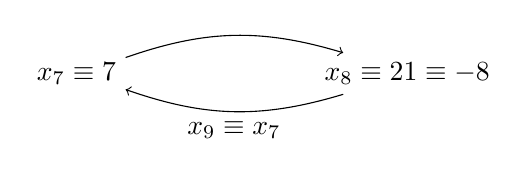
\begin{tikzpicture}
    \node (a) at (0,0) {$x_7\equiv 7$};
    \node (b) at (4.2,0) {$x_8\equiv 21\equiv -8$};
    \draw[->] (a) to[bend left=18] (b);
    \draw[->] (b) to[bend left=18] node[below] {$x_9\equiv x_7$} (a);
\end{tikzpicture}
\caption{The cycle found modulo $29$: the arrow in the notes identifies $x_9$ with $x_7$.}
\end{figure}

\begin{remark}
With $f(x)=x^2+1$, every term $x_i$ has to be stored before a useful divisor can be read off from a difference. (The formula $f(x)=x^2+1$ is struck through in the notes at this point.) The repair below tests only one difference per step.
\end{remark}

\paragraph{Repair.}
Replace the polynomial by $f(x)=x^2+c$ for a fixed integer $c$, and run two copies of the iteration from the same seed $x_0=y_0$:
\[
    x_{i+1}=f(x_i), \qquad y_{i+1}=f(f(y_i)).
\]
The fast copy is just the even terms of the slow copy, $y_i=x_{2i}$. At each step compute
\[
    \gcdop\bigl(|x_i-y_i|,\, N\bigr).
\]
If the gcd equals $1$, continue. If it equals $N$, change $f$ (a different $c$, or a different seed). If $1<\gcdop(|x_i-y_i|,N)<N$, the gcd is a factor of $N$.

\paragraph{Why the repair works.}
The sequence $(x_i)$, reduced modulo a factor $k$ of $N$, takes values in a finite set, so it is eventually periodic modulo $k$. There exist integers $T\ge 0$ and $M\ge 1$ such that
\begin{equation}
    x_{r+M}\equiv x_r\pmod{k}
    \qquad\text{for every }r\ge T.
    \label{eq:period}
\end{equation}

% --- page 29 ---

Now suppose $j>i$ and $x_j\equiv x_i\pmod{k}$. Then the indices have already passed the tail, so $i\ge T$, and they differ by a multiple of the period, $j\equiv i\pmod{M}$.

In particular,
\[
    x_{2i}\equiv x_i\pmod{k}
\]
as soon as $i\ge T$ and $2i\equiv i\pmod{M}$, that is $i\equiv 0\pmod{M}$. Among the $M$ consecutive integers
\[
    T,\; T+1,\; \ldots,\; T+M-1
\]
there is a multiple of $M$. That multiple is an admissible index (or the next multiple of $M$ is, which is at most $T+M$). For the corresponding $i$ one has $y_i=x_{2i}\equiv x_i\pmod{k}$, so $k$ divides $x_i-y_i$. Unless the same difference vanishes modulo $N$, the gcd with $N$ is a nontrivial factor.

\begin{theorem}
Let $S$ be a finite set with $m$ elements, let $f\colon S\to S$ be a map, and let $x_0\in S$. Write $x_i=f^{i}(x_0)$. Suppose there exist integers $T$ and $M$ such that
\[
    x_{r+M}=x_r \qquad\text{for every }r\ge T.
\]
Then $x_{2i}=x_i$ for some index $i$ with $1\le i\le T+M$.
\end{theorem}

\begin{remark}
% FIX p.29: the notes say ``if $f$ is sufficient'', which is read as ``sufficiently random''.
If $f$ is sufficiently random, then for large $m$ the expected value of the sum $T+M$ is about $1.253\sqrt{m}$. (The constant is $\sqrt{\pi/2}\approx 1.2533$, the expected length of the tail plus the cycle for a random function on a set of size $m$.)
\end{remark}

\subsection{Pollard's \texorpdfstring{$p-1$}{p-1} method}

This is the second of Pollard's algorithms. It is also the reason one has to be careful when choosing the secret primes in RSA.

Let $N=pq$ with $p$ and $q$ prime. If $p-1$ or $q-1$ factors into small primes, then $p$ and $q$ can be recovered from $N$.

Suppose there is an integer $L$ such that $(p-1)\mid L$ but $(q-1)\nmid L$. Write
\[
    L=(p-1)\,i
    = (q-1)\,j + k,
    \qquad 0<k<q-1.
\]

% --- page 30 ---

Take an integer $a$ with $\gcdop(a,N)=1$. Then $\gcdop(a,p)=\gcdop(a,q)=1$, and Fermat's theorem gives
\[
    a^{L}=(a^{p-1})^{i}\equiv 1\pmod{p},
\]
so $p$ divides $a^{L}-1$. On the other side,
\[
    a^{L}=a^{(q-1)j+k}=(a^{q-1})^{j}\,a^{k}\equiv a^{k}\pmod{q}.
\]
Hope that $a^{k}\not\equiv 1\pmod{q}$. Then $a^{L}\not\equiv 1\pmod{q}$, so $q$ does not divide $a^{L}-1$. Therefore
\[
    \gcdop(a^{L}-1,\, N)=p.
\]

\paragraph{How to choose $a$.}
The group $\units{q}$ has $\varphi(\varphi(q))$ primitive roots. For $q$ prime one has $\varphi(q)=q-1$, so this count is $\varphi(q-1)$. If $a$ is a primitive root modulo $q$, then $a^{k}\not\equiv 1\pmod{q}$ whenever $0<k<q-1$, and the hope above holds. The value $\varphi(q-1)$ is large when $q-1$ has no small prime factors, so in that case a random $a$ is reasonably likely to work. The running time is large when $p-1$ has a large prime factor, which is what one wants of an RSA prime.
% FIX p.30: the two facts are separate. A large $\varphi(q-1)$ makes a random base likely to satisfy $a^k\not\equiv 1\pmod q$. The cost is the size of the largest prime factor of $p-1$, not that count.

\paragraph{How to choose $L$.}
Suppose $p-1$ has only small prime factors. Then $(p-1)\mid n!$ for some $n$ that is still small, and
\[
    L=n!
\]
is a possible choice. One therefore tries to compute $\gcdop(a^{n!}-1,\, N)$, as follows.
\begin{itemize}[leftmargin=1.4em]
    \item Start with $a=2$.
    \item If the gcd equals $1$, increase $n$.
    \item If the gcd equals $N$, change $a$.
    \item If $1<\gcdop(a^{n!}-1,N)<N$, the gcd is a factor of $N$.
\end{itemize}

% --- page 31 ---

\paragraph{Method.}
Compute $\gcdop(a^{n!}-1,\, N)$ for various choices of $a$ and $n$. Each new factorial power is one extra exponentiation: $a^{(n+1)!}=(a^{n!})^{n+1}$.

\begin{example}
Take $N=9869$ and $a=2$. The successive values of $2^{n!}-1$, reduced modulo $N$ once they exceed $N$, are
\begin{center}
\begin{tabular}{c@{\qquad}c@{\qquad}c}
    $n$ & $2^{n!}-1 \bmod N$ & $\gcdop(2^{n!}-1,\, N)$\\[0.3em]
    $1$ & $2^{1}-1=1$ & $1$\\
    $2$ & $2^{2}-1=3$ & $1$\\
    $3$ & $2^{6}-1=63$ & $1$\\
    $4$ & $2^{24}-1\equiv 9784$ & $1$\\
    $5$ & $2^{120}-1\equiv 7491$ & $1$\\
    $6$ & $2^{6!}-1\equiv 9774$ & $1$\\
    $7$ & $2^{7!}-1\equiv 9443$ & $71$
\end{tabular}
\end{center}
% FIX p.31: the notes omit the factorial sign on the exponents $1,2,6,24,120$. Those are $1!$ through $5!$; the factorial sign appears explicitly from $6!$ onward. The residues above are the ones written in the notes ($2^{24}\equiv 9785$, so $2^{24}-1\equiv 9784$, and likewise for $2^{120}$, $2^{720}$ and $2^{5040}$).
Thus $\gcdop(9443,\, N)=71$. Dividing gives the complementary factor $9869/71=139$, and
\[
    N=71\cdot 139.
\]
The reason $n=7$ is the first success is visible in the factorizations
\[
    p-1=70=2\cdot 5\cdot 7, \qquad q-1=138=2\cdot 3\cdot 23.
\]
The prime $7$ divides $7!$ but not $6!$, so $70\mid 7!$ and $70\nmid n!$ for every $n<7$. The prime $23$ does not divide $7!$, so $138\nmid 7!$. This is exactly the situation $L=n!$ was chosen for.
\end{example}

\paragraph{Cost.}
A power $a^{k}\bmod N$ can be computed in $O(\log k)$ multiplications. Stirling's approximation gives
\begin{equation}
    \log(k!)
    = k\log k - k + \tfrac12\log(2\pi k) + O\bigl(\tfrac1k\bigr),
    \label{eq:stirling}
\end{equation}
so $\log(k!)=O(k\log k)$. Computing $a^{k!}\bmod N$ by fast exponentiation therefore takes $O(k\log k)$ steps.
% FIX p.31: the notes write $\log(k!)\simeq k\log k+\frac12\log(2\pi)+O(1/k)$, omitting the $-k$ term and the factor $k$ inside the logarithm. The $O(k\log k)$ bound uses only the leading term, so the conclusion is unchanged.

\section{Factorization via a Difference of Squares}
% ============================================================

The identity
\[
    x^2-y^2=(x-y)(x+y)
\]
turns a representation of $N$ as a difference of squares into a factorization. If $N=pq$ can be written $N=x^2-y^2$, then
\[
    N=(x+y)(x-y)
\]
and the two factors on the right are proper as soon as $x-y>1$.

% --- page 32 ---

\paragraph{Search.}
Given $N$, test $N+1^2$, $N+2^2$, $N+3^2$, \ldots\ until a square appears.

\begin{example}
Take $N=4331$.
\begin{align*}
    N+1^2 &= 4332 &&\text{(not a square)},\\
    N+2^2 &= 4335 &&\text{(not a square)},\\
    N+3^2 &= 4340 &&\text{(not a square)},\\
    N+4^2 &= 4347 &&\text{(not a square)},\\
    N+5^2 &= 4356 = 66^2.
\end{align*}
Therefore
\[
    N=66^2-5^2=(66-5)(66+5)=61\cdot 71.
\]
\end{example}

\begin{example}[Twin primes]
Let $p$ and $p+2$ both be prime, and set $N=p(p+2)$. Then
\[
    N+1^2=p^2+2p+1=(p+1)^2,
\]
so the search succeeds at the first step, and
\[
    N=\bigl((p+1)-1\bigr)\bigl((p+1)+1\bigr)=p(p+2).
\]
\end{example}

The same algebra applies to any odd product of two factors at a known distance. If $N=n(n+k)$ is odd, then both factors are odd, so $k$ is even and $k/2$ is an integer. Completing the square,
\[
    N+\Bigl(\frac{k}{2}\Bigr)^2
    = n(n+k)+\frac{k^2}{4}
    = \Bigl(n+\frac{k}{2}\Bigr)^2.
\]
Thus $N$ is a difference of squares with gap $k/2$, and Fermat's search stops by the time it reaches $N+(k/2)^2$.

The lesson for RSA is to take primes $p$ and $q$ of similar size, but not too close to each other. If $|p-q|=k$, it is enough to test
\[
    N+1^2,\; N+2^2,\; \ldots,\; N+\bigl(k/2\bigr)^2,
\]
which is only $k/2$ values.

% --- page 33 ---

\paragraph{A small multiplier.}
Writing $N$ itself as a difference of squares may fail for a long time; that attempt is crossed out in the notes. One looks instead for a small positive integer $k$ such that
\[
    kN=x^2-y^2=(x-y)(x+y),
\]
and hopes to recover the factors of $N$ from
\[
    \gcdop(N,\, x+y) \qquad\text{and}\qquad \gcdop(N,\, x-y).
\]

\begin{example}
Take $N=3589$. Then $\sqrt{N}\approx 60$, so a search for prime factors by trial division only has to inspect the $17$ primes up to $60$.
% FIX p.33: the notes write ``$17$ primes up to $160$''. There are $17$ primes at most $59$, and $37$ primes at most $160$. The previous line is $\sqrt{N}\approx 60$, so the bound is $60$.
Suppose $N+k^2$ is not a square for $k=1,\ldots,10$. Trying the multiplier $3$ instead,
\begin{align*}
    3N+1^2 &= 10768,\\
    3N+2^2 &= 10771,\\
    3N+3^2 &= 10776,\\
    3N+4^2 &= 10783,\\
    3N+5^2 &= 10792,\\
    3N+6^2 &= 10803,\\
    3N+7^2 &= 10816 = 104^2.
\end{align*}
(Here $3N=3\cdot 3589=10767$, and $10767+49=10816$.) Therefore
\begin{align*}
    3N &= 104^2-7^2=(104-7)(104+7)=97\cdot 111.
\end{align*}
Since $111=3\cdot 37$,
\[
    N=97\cdot 37.
\]
Both $97$ and $37$ are prime. Searching through $N+k^2$ was the tedious option; $3N+k^2$ succeeded.
\end{example}

The same idea with multiplier $2$ is a natural question: what about $2N+k^2$? Keep in mind that one still wants
\[
    N=pq=(x+y)(x-y)
\]
after removing the extra factor of $2$.

% --- page 34 ---

It never works for odd $N$. Squares modulo $4$ are $0$ or $1$, and an odd $N$ satisfies $2N\equiv 2\pmod{4}$, so
\[
    k^2\equiv 0\text{ or }1\pmod{4}
    \qquad\text{and}\qquad
    2N+k^2\equiv 2\text{ or }3\pmod{4}.
\]
A square cannot be $2$ or $3$ modulo $4$, hence $2N+k^2$ is never a square.

\lectureheading{Lecture 18 (16/10/26)}

\section{RSA Encryption}
% ============================================================

This is a recall of the scheme. Alice creates a key, split into a public half and a private half. Bob uses the public half to encrypt a message; Alice uses the private half to decrypt it. The channel between them is insecure. Bob's goal is to send Alice a message in encrypted form.

\begin{figure}[H]
\centering
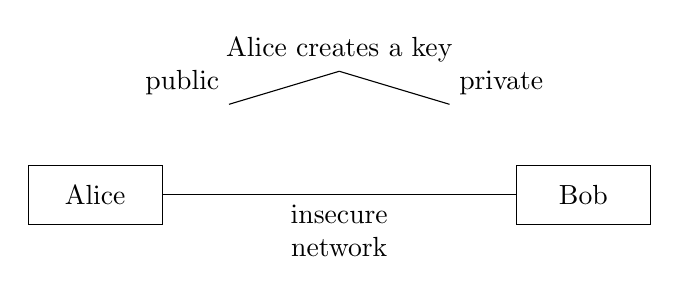
\begin{tikzpicture}[every node/.style={font=\normalsize}]
    \node[draw, minimum width=1.7cm, minimum height=0.75cm] (A) at (0,0) {Alice};
    \node[draw, minimum width=1.7cm, minimum height=0.75cm] (B) at (6.2,0) {Bob};
    \draw (A.east) -- (B.west);
    \node[align=center, below] at (3.1,0) {insecure\\ network};
    \node[align=center] (key) at (3.1,1.85) {Alice creates a key};
    \draw (key.south) -- (1.7,1.15) node[above left] {public};
    \draw (key.south) -- (4.5,1.15) node[above right] {private};
\end{tikzpicture}
\caption{Alice publishes one half of her key. Bob encrypts with the public half; only Alice's private half decrypts. The network between them is insecure.}
\end{figure}

The protocol rests on the difficulty of solving
\[
    x^{e}\equiv C\pmod{N}
\]
for $x$, when $C$, $e$ and $N$ are given.

\paragraph{Step 1: key generation (Alice).}
Alice chooses primes $p$ and $q$, and an encryption exponent $e$. She computes
\[
    N=pq, \qquad \varphi(N)=(p-1)(q-1).
\]

% --- page 35 ---

The exponent $e$ must be coprime to $\varphi(N)$, and the decryption exponent $d$ is its inverse:
\[
    de\equiv 1\pmod{\varphi(N)}.
\]
Alice publishes the public key $(e,N)$ and keeps the private key $(p,q,d)$.

\paragraph{Step 2: encryption (Bob).}
The message is an integer $m$ with $0\le m<N$. Bob computes
\[
    m^{e}\equiv C\pmod{N}
\]
and sends the ciphertext to Alice: $m^{e}\equiv C\pmod{N}$.

\paragraph{Step 3: decryption (Alice).}
Alice computes
\[
    C^{d}\equiv m^{ed}\equiv m\pmod{N},
\]
where the last step is Euler's theorem (or the Chinese remainder theorem, if $\gcdop(m,N)>1$): since $ed=1+\varphi(N)\,t$ for some integer $t$, one has $m^{ed}=m\cdot(m^{\varphi(N)})^{t}\equiv m\pmod{N}$ whenever $\gcdop(m,N)=1$.

\paragraph{When is RSA hard to break?}
The factorization attacks above impose three conditions.
\begin{enumerate}[leftmargin=1.6em]
    \item $p\sim q$, that is, $p$ and $q$ are of about the same size.
    \item $p$ and $q$ should not be too close. (A twin prime is the extreme case: Fermat's search then stops at $N+1^2$.)
    % FIX p.35: ``not'' is inserted with a caret, so that the line reads ``should not be too close'' rather than ``should be too close''.
    \item $p-1$ and $q-1$ should not have very small prime factors. (A Fermat prime is a bad choice: if $p=2^{2^{r}}+1$, then $p-1$ is a power of $2$, and Pollard's $p-1$ method applies.)
\end{enumerate}
% UNCLEAR p.35: a circled mark under item~3 is scribbled out; no fourth condition is readable.

\section{Implementation and Security Issues}
% ============================================================

\subsection{A man-in-the-middle attack}

The attack uses an active adversary on the insecure network, rather than a passive eavesdropper.

\begin{figure}[H]
\centering
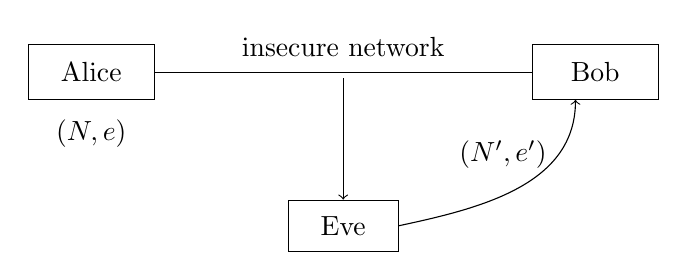
\begin{tikzpicture}
    \node[draw, minimum width=1.6cm, minimum height=0.7cm] (A) at (0,0) {Alice};
    \node[draw, minimum width=1.6cm, minimum height=0.7cm] (B) at (6.4,0) {Bob};
    \draw (A.east) -- (B.west);
    \node[above] at (3.2,0.08) {insecure network};
    \node[anchor=north] at (0,-0.48) {$(N,e)$};
    \node[draw, minimum width=1.4cm, minimum height=0.65cm] (E) at (3.2,-1.95) {Eve};
    \draw[->] (3.2,-0.08) -- (E.north);
    \draw[->] (E.east) to[out=12,in=-90] (6.15,-0.35);
    \node[anchor=west] at (4.55,-1.05) {$(N',e')$};
\end{tikzpicture}
\caption{Eve sits on the channel. She sees Alice's public key $(N,e)$ and substitutes her own key $(N',e')$ on the way to Bob.}
\end{figure}

% --- page 36 ---

Eve has complete control of the insecure network.
\begin{enumerate}[leftmargin=1.6em]
    \item Eve sends Bob a public key $(N',e')$ of her own, in place of Alice's key $(N,e)$. Bob, intending to send a message $m$ to Alice, computes
    \[
        m^{e'}\equiv C'\pmod{N'}
    \]
    and tries to send the ciphertext $C'$ to Alice.
    \item Eve intercepts $C'$. She holds the decryption exponent $d'$ for her own modulus, so
    \[
        (C')^{d'}\equiv (m^{e'})^{d'}\equiv m\pmod{N'}.
    \]
    She then re-encrypts the plaintext under Alice's genuine public key,
    \[
        m^{e}\equiv C\pmod{N},
    \]
    and forwards $C$ to Alice. Alice's decryption recovers the message,
    \[
        C^{d}\equiv m^{ed}\equiv m\pmod{N}.
    \]
\end{enumerate}
Alice receives Bob's message, and at the same time Eve knows it. This is a \emph{man-in-the-middle} attack, also called an \emph{impersonation} attack.

% --- page 37 ---

\subsection{A chosen-ciphertext attack}

\paragraph{Assumption.}
Eve can manipulate Alice.
Listening on the channel, by contrast, is always available to her.

\begin{figure}[H]
\centering
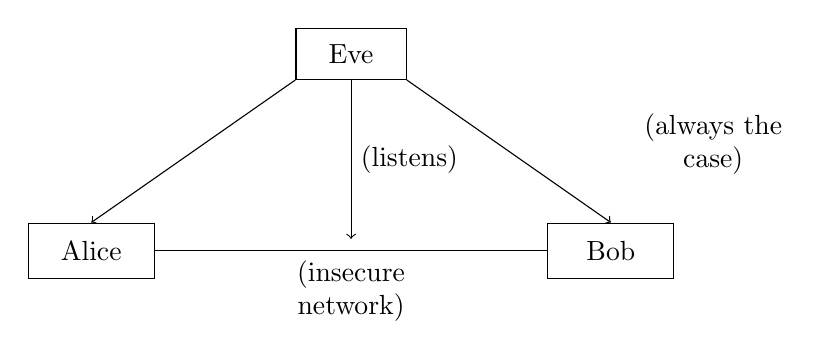
\begin{tikzpicture}
    \node[draw, minimum width=1.4cm, minimum height=0.65cm] (E) at (3.3,2.5) {Eve};
    \node[draw, minimum width=1.6cm, minimum height=0.7cm] (A) at (0,0) {Alice};
    \node[draw, minimum width=1.6cm, minimum height=0.7cm] (B) at (6.6,0) {Bob};
    \draw (A.east) -- (B.west);
    \node[align=center, below] at (3.3,0) {(insecure\\ network)};
    \draw[->] (E.south west) -- (A.north);
    \draw[->] (E.south) -- (3.3,0.15) node[midway, right] {(listens)};
    \draw[->] (E.south east) -- (B.north);
    \node[align=center, anchor=west] at (6.9,1.35) {(always the\\ case)};
\end{tikzpicture}
\caption{Chosen-ciphertext setting. Eve listens on the channel between Alice and Bob (that direction is always open) and can also send messages to Alice.}
\end{figure}

\begin{enumerate}[leftmargin=1.6em]
    \item \textbf{Key generation.}
    Alice's public key is $(N,e)$ and her private key is $(p,q,d)$.
    \item \textbf{Encryption.}
    Let $m$ be the message. Bob sends
    \[
        m^{e}\equiv C\pmod{N}
    \]
    to Alice, and Eve sees $C$. Eve then asks Alice to verify herself, and Alice agrees. Eve chooses an integer $k$ with $1<k<N$ and $\gcdop(k,N)=1$, and sends Alice the altered ciphertext
    \[
        m'\equiv C\,k^{e}\pmod{N}.
    \]
    Alice decrypts and returns
    \[
        S\equiv (m')^{d}\pmod{N}
    \]
    to Eve. Expanding the power,
    \begin{align*}
        (C\,k^{e})^{d}
        &\equiv (m^{e}\,k^{e})^{d}
        \equiv (mk)^{ed}
        \equiv mk \pmod{N}.
    \end{align*}
    So the value Alice sends back is $S\equiv mk\pmod{N}$.
\end{enumerate}

% CONTINUES: chosen-ciphertext attack on textbook RSA
% --- page 38 ---

Eve chose $k$ with $\gcdop(k,N)=1$ and obtained Alice's decryption
$S\equiv mk\pmod{N}$ of the blinded ciphertext. Multiplying by the
inverse of $k$ removes the blinding factor:
\[
    m\equiv (mk)\,k^{-1}\pmod{N}.
\]
Bob's ciphertext was $C\equiv m^{e}\pmod{N}$. Eve will send that same
ciphertext on to Alice,
\[
    m^{e}\equiv C\pmod{N}.
\]
Both Alice and Eve have Bob's message.

The attack used two facts about textbook RSA: encryption is deterministic,
and Alice was willing to decrypt a ciphertext Eve had chosen.

\paragraph{Question.}
What is the way out of these attacks?

\paragraph{Answer.}
Use RSA--OAEP (Optimal Asymmetric Encryption Padding). Alice's public key
is still $(N,e)$ and her private key is still $(p,q,d)$, but she asks Bob
to send the message in a prescribed form. A padding block is attached to
the message,
\[
    m'
    =
    \begin{array}{|c|c|}
        \hline
        m & \text{Padding}\\
        \hline
    \end{array},
\]
and Bob encrypts the whole block,
\[
    (m')^{e}
    \equiv
    \Biggl(
        \begin{array}{|c|c|}
            \hline
            m & \text{Padding}\\
            \hline
        \end{array}
    \Biggr)^{e}
    \pmod{N}.
\]
Alice decrypts and recovers the block, not a bare integer:
\[
    (m')^{ed}
    \equiv
    \begin{array}{|c|c|}
        \hline
        m & \text{Padding}\\
        \hline
    \end{array}
    \pmod{N}.
\]
% FIX p.38: an intermediate line wrote $(m')^{ed}\equiv m\pmod{N}$.
% The next line corrects it: decryption returns the padded block.
If the padding is still in its original form, she accepts the message and
the line is treated as secure; otherwise she rejects it.

% --- page 39 ---

\begin{example}[Secret bids for a house]
Alice is accepting secret bids for a house. Her RSA key is
\[
    (N,e)=(77,7),
    \qquad
    (p,q,d)=(7,11,43).
\]
% filled in: $7\cdot 43=301=5\cdot 60+1$, so $ed\equiv 1\pmod{\varphi(N)}$
% with $\varphi(77)=60$.
The bidders are Eve and Bob.

\begin{figure}[H]
\centering
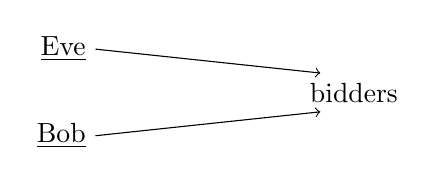
\begin{tikzpicture}[every node/.style={font=\normalsize}]
    \node[anchor=east] (eve) at (0,0.55) {\underline{Eve}};
    \node[anchor=east] (bob) at (0,-0.55) {\underline{Bob}};
    \node[anchor=west] (bid) at (2.6,0) {bidders};
    \draw[->] (eve.east) -- (bid.150);
    \draw[->] (bob.east) -- (bid.210);
\end{tikzpicture}
\caption{Eve and Bob are the two bidders.}
\end{figure}

Eve's plan: whatever Bob bids, she wants to bid double that amount.

Let Bob's secret bid be $m_{B}=5$. Alice receives
\[
    C_{B}\equiv m_{B}^{7}\pmod{77}.
\]
% filled in: $5^{7}=78125\equiv 47\pmod{77}$, so $C_{B}\equiv 47$.
\begingroup\samepage
Eve takes $k=2$ and builds a ciphertext for twice the bid, using the
public exponent on the multiplier:
\begin{align*}
    C_{E}
    &\equiv 2^{e}\,C_{B}\pmod{N}\\
    &\equiv 2^{7}\cdot 47
     \equiv 10\pmod{77}.
\end{align*}
\endgroup
% FIX p.39: the notes label this ciphertext $m_{E}$. It is $C_{E}$.
Alice decrypts Bob's ciphertext and recovers his bid:
\[
    m_{B}
    \equiv C_{B}^{d}
    \equiv m_{B}^{7d}
    \equiv 5\pmod{N}.
\]
Decrypting Eve's ciphertext gives
\[
    M_{E}
    \equiv C_{E}^{d}
    \equiv 2\,m_{B}
    \equiv 10\pmod{N}.
\]
% FIX p.39: the notes write $C_{E}^{d}=2^{e}\,C_{B}^{e}$. The right-hand
% side is not the decryption; $C_{E}\equiv 2^{e}C_{B}$ decrypts to $2m_{B}$.
% (In this tiny modulus one also has $10^{7}\equiv 10\pmod{77}$, so the
% ciphertext residue and the plaintext happen to coincide.)
Without padding, Eve's bid is exactly double Bob's, and Alice cannot tell
that the second ciphertext was manufactured from the first.

Alice therefore demands a check digit. A bid is sent as the block
$\begin{array}{|c|c|}\hline m & 1\\\hline\end{array}$.
Then
\begin{align*}
    C_{B}
    &\equiv
    \Biggl(
        \begin{array}{|c|c|}
            \hline
            m & 1\\
            \hline
        \end{array}
    \Biggr)^{e}
    \pmod{N},\\[0.4em]
    C_{E}
    &\equiv
    2^{e}
    \Biggl(
        \begin{array}{|c|c|}
            \hline
            m & 1\\
            \hline
        \end{array}
    \Biggr)^{e}
    \equiv
    \Biggl(
        2\cdot
        \begin{array}{|c|c|}
            \hline
            m & 1\\
            \hline
        \end{array}
    \Biggr)^{e}
    \pmod{N}.
\end{align*}
The integer inside Eve's power is Bob's block multiplied by $2$. In the
schematic of the notes that product is a block ending in $0$,
\[
    \begin{array}{|c|c|}
        \hline
        m_{E} & 0\\
        \hline
    \end{array},
\]
rather than a block ending in the check digit $1$.
% FIX p.39: the notes equate $C_{E}$ itself with the block $|m_{E}|0|$.
% That block is the plaintext Eve's ciphertext decrypts to.
\end{example}

% --- page 40 ---

Alice decrypts Bob's ciphertext and sees the check digit she asked for:
\begin{align*}
    M_{B}
    &\equiv C_{B}^{d}\pmod{N}\\
    &\equiv
    \Biggl(
        \begin{array}{|c|c|}
            \hline
            m & 1\\
            \hline
        \end{array}
    \Biggr)^{ed}
    \equiv
    \begin{array}{|c|c|}
        \hline
        m & 1\\
        \hline
    \end{array}
    \pmod{N}.
\end{align*}
% FIX p.40: the first line was written $M_{B}\equiv C_{B}\pmod{N}$,
% without the decryption exponent. The next line has the exponent $ed$.
Bob's bid is accepted. Eve's ciphertext decrypts to
\begin{align*}
    C_{E}^{d}
    &\equiv
    \Biggl(
        \begin{array}{|c|c|c|}
            \hline
            2 & m & 1\\
            \hline
        \end{array}
    \Biggr)^{ed}
    \equiv
    \begin{array}{|c|c|}
        \hline
        2m & 0\\
        \hline
    \end{array}
    \pmod{N}.
\end{align*}
The check digit is no longer $1$, so Alice rejects Eve's bid.

Suppose the padding has $216$ digits. The chance that multiplication
leaves that same padding is
\[
    \frac{1}{2^{216}},
\]
which is insignificant.
% UNCLEAR p.40: the length is written ``216 digits'', but the probability
% is $1/2^{216}$ (the count one would write for $216$ bits). Left as written.

% ============================================================
\section{Digital Signatures}
% ============================================================

Encryption is about secrecy: the message should not leak. A digital
signature is about authenticity of the message and of the sender.

A physical signature does not give that guarantee. On a degree
certificate the same handwritten signature can be copied from one line
to another.

\begin{figure}[H]
\centering
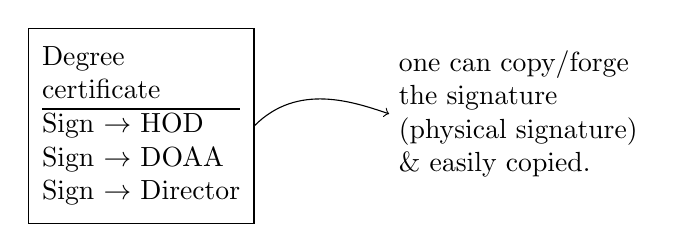
\begin{tikzpicture}[font=\normalsize]
    \node[draw, align=left, inner sep=5pt] (cert) at (0,0) {%
        \begin{tabular}{@{}l@{}}
            Degree\\
            certificate\\
            \hline
            Sign $\rightarrow$ HOD\\
            Sign $\rightarrow$ DOAA\\
            Sign $\rightarrow$ Director
        \end{tabular}};
    \node[align=left, anchor=west] (note) at (3.15,0.15)
        {one can copy/forge\\
         the signature\\
         (physical signature)\\
         \& easily copied.};
    \draw[->] (cert.east) .. controls +(0.55,0.55) and +(-0.45,0.15) .. (note.west);
\end{tikzpicture}
\caption{A physical signature on a degree certificate can be copied.}
\end{figure}

% --- page 41 ---

Three properties are required of a signature scheme.

\begin{enumerate}[leftmargin=1.6em]
    \item One wants an algorithm by which the signature cannot be copied
    or forged the way a physical signature can.

    \begin{figure}[H]
    \centering
    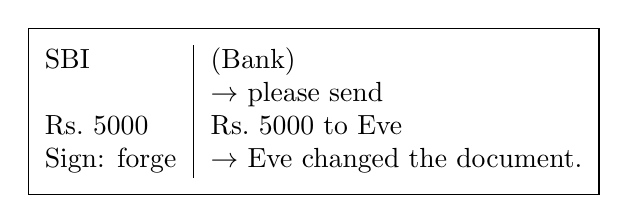
\begin{tikzpicture}[font=\normalsize]
        \node[draw, inner sep=6pt] {%
            \begin{tabular}{@{}l|l@{}}
                SBI & (Bank)\\
                & $\rightarrow$ please send\\
                Rs.\ 5000 & Rs.\ 5000 to Eve\\
                Sign: forge & $\rightarrow$ Eve changed the document.
            \end{tabular}};
    \end{tikzpicture}
    \caption{A forged signature on an altered bank instruction.}
    \end{figure}
    % UNCLEAR p.41: the amount cell reads roughly ``SSS 5000'' with a
    % rupee-like mark. Taken as Rs.\ 5000, and the annotation as
    % ``Rs.\ 5000 to Eve''.

    The picture is an instruction to SBI. Eve alters the document so that
    it says ``please send Rs.\ 5000 to Eve'' and forges the signature. A
    digital signature has to make that alteration detectable.

    \item In the signed copy, one cannot change the message. If Eve's
    change succeeds and the bank has transferred the money to Eve's
    account, Alice can deny that she signed the document. The signature
    must bind her to the text that was actually signed.

    \item \emph{Non-repudiation}: once Alice has signed, she cannot later
    deny the signature.
\end{enumerate}

% ------------------------------------------------------------
\subsection{RSA signatures}
% ------------------------------------------------------------

\begin{keybox}[title=RSA signatures]
\paragraph{Key generation (Alice).}
Alice chooses primes $p$ and $q$, sets $N=pq$, and chooses a verification
exponent $e$ with $\gcdop(e,\varphi(N))=1$. The signing exponent $d$ is
the inverse of $e$ modulo $\varphi(N)$, so $ed\equiv 1\pmod{\varphi(N)}$.
The public verification key is $(N,e)$; the private signing key is $d$.
Signing the document requires the private key.

% --- page 42 ---

Let $D$ be the document Alice wants to sign, read as an integer modulo $N$.

\paragraph{Signing.}
Alice computes
\[
    D^{\mathrm{sign}}\equiv D^{d}\pmod{N}
\]
and sends the pair $(D,D^{\mathrm{sign}})$ to Bob.

\paragraph{Verification.}
Bob computes $(D^{\mathrm{sign}})^{e}\pmod{N}$. Since
$ed\equiv 1\pmod{\varphi(N)}$,
\[
    (D^{\mathrm{sign}})^{e}
    \equiv D^{de}
    \equiv D\pmod{N}
\]
whenever $\gcdop(D,N)=1$. He accepts the signature when the power equals
$D$, and rejects it otherwise:
\[
    (D^{\mathrm{sign}})^{e}
    \equiv
    \begin{cases}
        D\pmod{N} & \text{true (accept)},\\
        \neq D\pmod{N} & \text{false (reject)}.
    \end{cases}
\]
\end{keybox}

\begin{example}[A small RSA signature]
Take $p=5$, $q=11$, so $N=55$ and $\varphi(N)=40$. Let $e=3$ and let the
document be $D=7$. The notes ask to verify the scheme on these values.

The signing exponent satisfies $3d\equiv 1\pmod{40}$. Since
$3\cdot 27=81\equiv 1\pmod{40}$, one may take $d=27$. Then
\begin{align*}
    7^{2}&\equiv 49,\\
    7^{3}&\equiv 13,\\
    7^{6}&\equiv 13^{2}=169\equiv 4,\\
    7^{12}&\equiv 16,\\
    7^{24}&\equiv 256\equiv 36\pmod{55},
\end{align*}
and
\[
    D^{\mathrm{sign}}
    \equiv 7^{27}
    \equiv 7^{24}\cdot 7^{2}\cdot 7
    \equiv 36\cdot 49\cdot 7
    \equiv 28\pmod{55}.
\]
Verification:
\[
    28^{3}=21952\equiv 7\pmod{55},
\]
which equals $D$, so Bob accepts.
% filled in: the notes set $p,q,N,\varphi(N),e,D$ and say ``verify'',
% without computing $d$ or $D^{\mathrm{sign}}$.
\end{example}

% ------------------------------------------------------------
\subsection{ElGamal signatures}
% ------------------------------------------------------------

In practice one uses a modified ElGamal signature, the Digital Signature
Algorithm (DSA), to sign documents.
% FIX p.42: the notes expand DSA as ``Digital Signing Algorithm''.

The construction is based on the discrete logarithm, as opposed to the
RSA power. The contrast drawn on the page is
\begin{align*}
    x^{e}&\equiv C\pmod{N}
        &&\text{is the RSA relation},\\
    g^{x}&\equiv C\pmod{N}
        &&\text{is the discrete-logarithm relation}.
\end{align*}

% --- page 43 ---

The signature reuses ElGamal encryption from Lecture~12: Bob sends and Alice receives.

\paragraph{Key generation.}
Alice chooses a large prime $p$, a base $g\in\units{p}$ of large order, and a private exponent $a\in\Z$. She computes
\[
    A\equiv g^{a}\pmod{p},
\]
publishes the public key $(A,g,p)$, and keeps the private key $a$.

\paragraph{Encryption.}
For a message $m$, Bob chooses an exponent $b$ satisfying
\[
    1<b\le p-1,
    \qquad
    \gcdop(b,p-1)=1,
\]
computes
\begin{align*}
    c_{1}&\equiv g^{b}\pmod{p},\\
    c_{2}&\equiv m\,A^{b}\pmod{p},
\end{align*}
and sends $(c_{1},c_{2})$ to Alice.

\paragraph{Decryption.}
Alice computes $x\equiv c_{1}^{a}\pmod{p}$ and $x^{-1}\pmod{p}$. Then
\begin{align*}
    x^{-1}c_{2}
    &\equiv c_{1}^{-a}\,m\,A^{b}
     \equiv g^{-ab}\,m\,g^{ab}
     \equiv m\pmod{p}.
\end{align*}
% p.43: board says ``large order'', public key $(A,g,p)$, and $a\in\Z$
% with no written range. Bob's exponent is $1<b\le p-1$ and $\gcd(b,p-1)=1$.

% --- page 44 ---

\paragraph{Signing a document.}
\begin{enumerate}[leftmargin=1.6em]
    \item Alice chooses $(p,g,a)$ as above, publishes $(A,p,g)$, and
    keeps $a$.

    \item To sign a document $D$ with $1<D<p$, she chooses an integer $k$
    satisfying
    \[
        \gcdop(k,p-1)=1,
        \qquad
        1<k<p,
    \]
    and sets
    \begin{align*}
        s_{1}&\equiv g^{k}\pmod{p},\\
        s_{2}&\equiv (D-as_{1})\,k^{-1}\pmod{p-1}.
    \end{align*}
    The inverse exists because $k$ is coprime to $p-1$. She sends
    $(D,s_{1},s_{2})$ to Bob.

    \item Bob computes $A^{s_{1}}s_{1}^{s_{2}}\pmod{p}$ and compares it
    with $g^{D}$:
    \[
        A^{s_{1}}s_{1}^{s_{2}}
        \equiv
        \begin{cases}
            g^{D}\pmod{p} & \text{true (accept)},\\
            \neq g^{D}\pmod{p} & \text{false (reject)}.
        \end{cases}
    \]
\end{enumerate}

The test accepts an honestly produced signature. Indeed, writing the
exponents modulo $p-1$ and using $g^{p-1}\equiv 1\pmod{p}$,
\begin{align*}
    A^{s_{1}}s_{1}^{s_{2}}
    &\equiv (g^{a})^{s_{1}}(g^{k})^{s_{2}}
     \equiv g^{as_{1}+ks_{2}}\pmod{p}\\
    &\equiv g^{as_{1}+(D-as_{1})}
     \equiv g^{D}\pmod{p},
\end{align*}
because $ks_{2}\equiv D-as_{1}\pmod{p-1}$.
% filled in: the notes state the accept/reject test without this expansion.

\lectureheading{Lecture 19 (23/10/26)}

% ============================================================
\section{Factorization via a Difference of Squares}
% ============================================================

The aim is to write the composite modulus as a difference of squares.
From $x^{2}-y^{2}=(x+y)(x-y)$ one wants integers $a>b>0$ with
\[
    N=(a-b)(a+b)=a^{2}-b^{2}.
\]
The two factors are then $a-b$ and $a+b$.

% --- page 45 ---

One keeps a reasonable distance between $a$ and $b$: if they are very
close, then $a-b$ is small and the factorization is easy to find by
trying.

If $N$ itself is hard to write as a difference of two squares, try the
same idea on a multiple. For some positive integer $k$, write
\[
    kN=(a-b)(a+b)=a^{2}-b^{2}.
\]
Any prime factor of $N$ then divides $a-b$ or $a+b$, and
$\gcdop(N,a-b)$ or $\gcdop(N,a+b)$ can be a proper factor.

Equivalently, one looks for $a$ and $b$ with
\[
    a^{2}-b^{2}\equiv 0\pmod{N},
    \qquad\text{i.e.}\qquad
    a^{2}\equiv b^{2}\pmod{N},
\]
and $a\not\equiv \pm b\pmod{N}$. Searching for such a pair at random is
hard. The following strategy builds the congruence out of several easier
ones.

\paragraph{Step 1.}
Find integers $a_{1},\ldots,a_{n}$ such that
\[
    a_{i}^{2}\equiv c_{i}\pmod{N},
\]
and each $c_{i}$ has only small prime factors.

\paragraph{Step 2.}
Choose a subset of these relations, say
$a_{n_{1}},\ldots,a_{n_{k}}$, whose corresponding residues multiply to a
square:
\[
    c_{n_{1}}\cdots c_{n_{k}}=b^{2}
\]
for some integer $b$. The product of the $a_{n_{j}}$ then satisfies
\[
    a^{2}
    =(a_{n_{1}}\cdots a_{n_{k}})^{2}
    \equiv b^{2}\pmod{N},
    \qquad
    a\equiv a_{n_{1}}\cdots a_{n_{k}}\pmod{N}.
\]

\paragraph{Step 3.}
Compute $\gcdop(N,a-b)$ or $\gcdop(N,a+b)$. Either gcd is a factor of $N$.
It is a proper factor precisely when $a\not\equiv \pm b\pmod{N}$.

% --- page 46 ---

\begin{example}[$N=3589$]
Take $N=3589=37\cdot 97$, so $\sqrt{N}\approx 59.9$ and one starts the
search just above $60$.
\begin{align*}
    60^{2}&=3600\equiv 11\pmod{N},\\
    61^{2}&=3721\equiv 132=2^{2}\cdot 3\cdot 11\pmod{N},\\
    64^{2}&=4096\equiv 507=3\cdot 13^{2}\pmod{N}.
\end{align*}
The product of the three residues is a square:
\[
    (60\cdot 61\cdot 64)^{2}
    \equiv 2^{2}\cdot 3^{2}\cdot 11^{2}\cdot 13^{2}\pmod{N}.
\]
Hence
\begin{align*}
    a&\equiv 60\cdot 61\cdot 64\equiv 955\pmod{N},\\
    b&=2\cdot 3\cdot 11\cdot 13=858.
\end{align*}
% filled in: $60\cdot 61=3660\equiv 71$ and $71\cdot 64=4544\equiv 955\pmod{3589}$.
Now $a-b=955-858=97$, and
\[
    \gcdop(N,a-b)=\gcdop(3589,97)=97,
\]
which is a prime factor of $N$. The complementary factor is
$N/97=37$. Equivalently,
\[
    a+b=1813
    \qquad\text{and}\qquad
    \gcdop(N,a+b)=37.
\]
% filled in: the notes record only $\gcdop(N,a-b)=97$.
\end{example}

\begin{remark}
The gcd may be trivial: $\gcdop(a\pm b,N)\in\{1,N\}$. In that case the
pair $(a,b)$ came from a combination with $a\equiv \pm b\pmod{N}$, and
one tries a different combination of the $a_{i}$. The residues $c_{i}$
have to be chosen so that they have small prime factors; otherwise the
search for a product that is a square does not get off the ground.
\end{remark}

\begin{definition}[Smooth numbers]
Let $B\ge 2$ be an integer. An integer $n\ge 2$ is \emph{$B$-smooth} if
every prime factor of $n$ is at most $B$.
\end{definition}

% --- page 47 ---

\begin{example}[$7$-smooth numbers up to $40$]
The $7$-smooth integers from $2$ to $40$ are
\begin{align*}
    &2,3,4,5,6,7,8,9,10,12,14,15,16,18,20,\\
    &21,24,25,27,28,30,32,35,36,40.
\end{align*}
The integers from $2$ to $40$ that are not $7$-smooth are
\begin{align*}
    &11,13,17,19,22,23,26,29,31,33,34,\\
    &37,38,39.
\end{align*}
There are $25$ numbers in the first list and $14$ in the second.
\end{example}

These numbers have to be counted, for the following reason. Suppose
relations
\[
    a_{1}^{2}\equiv c_{1},\quad
    a_{2}^{2}\equiv c_{2},\quad
    \ldots,\quad
    a_{n}^{2}\equiv c_{n}\pmod{N}
\]
have been found, and each $c_{i}$ factors over a fixed set of small
primes. Let
\[
    \{p_{1},\ldots,p_{t}\}
\]
be the first $t$ primes (the factor base), and write
\[
    c_{i}=p_{1}^{e_{1i}}\cdots p_{t}^{e_{ti}},
    \qquad 1\le i\le n.
\]
A subset of the relations multiplies to a square precisely when there
are exponents $u_{i}\in\{0,1\}$ such that
\[
    c_{1}^{u_{1}}\cdots c_{n}^{u_{n}}
\]
is a square. The choice $u_{i}=0$ leaves $c_{i}$ out of the product, and
$u_{i}=1$ puts it in. Expanding the product,
\begin{align*}
    c_{1}^{u_{1}}\cdots c_{n}^{u_{n}}
    &=
    p_{1}^{u_{1}e_{11}+u_{2}e_{12}+\cdots+u_{n}e_{1n}}\\
    &\qquad\cdots\;
    p_{t}^{u_{1}e_{t1}+u_{2}e_{t2}+\cdots+u_{n}e_{tn}}.
\end{align*}

% --- page 48 ---

The product is a square if and only if every exponent is even:
\begin{align*}
    u_{1}e_{11}+u_{2}e_{12}+\cdots+u_{n}e_{1n}
        &\equiv 0\pmod{2},\\
    &\vdots\\
    u_{1}e_{t1}+u_{2}e_{t2}+\cdots+u_{n}e_{tn}
        &\equiv 0\pmod{2}.
\end{align*}
This is a homogeneous linear system of $t$ equations in the $n$ unknowns
$u_{1},\ldots,u_{n}$, over the field $\Z/2\Z$. A homogeneous system with
more unknowns than equations has a non-trivial solution, so a non-trivial
solution exists whenever $n>t$.

The factor base is the set of the first $t$ primes, and $p_{t}$ is the
$t$-th prime, so $\pi(p_{t})=t$. The same demand can therefore be written
\[
    n>\pi(p_{t}):
\]
one needs more smooth relations than there are primes up to the
smoothness bound. To know whether a chosen bound produces that many
relations, one needs a count of smooth numbers.

\begin{definition}[Smooth-number counting function]
For $x\ge 1$ and an integer $B\ge 2$,
\[
    \psi(x,B)
    =
    \#\{\,n : 1<n\le x,\ n\text{ is $B$-smooth}\,\}.
\]
\end{definition}

\begin{example}
From the lists above, $\psi(20,7)=15$ and $\psi(40,7)=25$.
\end{example}

The two arguments have to be related before the count is useful as an
estimate. If $B>x$, every integer $n$ with $2\le n\le x$ is $B$-smooth,
because every prime factor of $n$ is at most $n\le x<B$. The definition
excludes $n=1$, so
\[
    \psi(x,B)=x-1
    \qquad\text{whenever }B>x
\]
(and $x$ is an integer). In the factorization one varies $x$ and $B$
together. Set
\[
    u=\frac{\log x}{\log B},
    \qquad\text{equivalently}\qquad
    B=x^{1/u}.
\]

% --- page 49 ---

\begin{keybox}
\begin{theorem}[Canfield--Erd\H{o}s--Pomerance]
Fix $0<\varepsilon<1/2$, and let $x$ and $B$ satisfy
\[
    (\log x)^{\varepsilon}
    <
    \log B
    <
    (\log x)^{1-\varepsilon}.
\]
Let $u=\log x/\log B$. Then
\[
    \psi(x,B)
    =
    x\,u^{-u\bigl(1+o(1)\bigr)}
    \qquad\text{as }x\to\infty.
\]
\end{theorem}
\end{keybox}
% FIX p.49: the notes spell the first name ``Caufield''.

\begin{remark}
The symbol $o(1)$ stands for a function of $x$ which tends to $0$ as
$x\to\infty$.
\end{remark}

To use $\psi(x,B)$ one still has to choose $B$. Define
\[
    L(x)
    =
    \exp\Bigl(\sqrt{\log x\cdot\log\log x}\Bigr).
\]
For every $m>0$ and every $\delta>0$, and for all sufficiently large $x$,
\[
    (\log x)^{m}<L(x)<x^{\delta}.
\]
% FIX p.49: the notes write both bounds with the side condition ``for $m>0$''
% and do not quantify $\delta$. The upper bound holds for every $\delta>0$.
In the order of growth this is the sandwich
\[
    (\log x)^{m}
    \;<\;
    \square
    \;<\;
    x^{\delta},
\]
with $L(x)$ an example of the middle term. A quantity of that shape is
called \emph{sub-exponential}.

\begin{figure}[H]
\centering
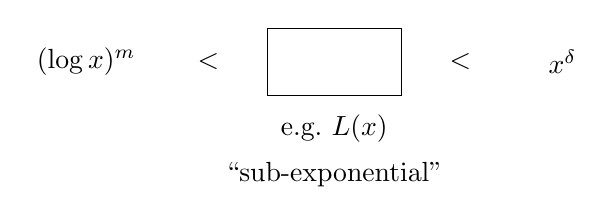
\begin{tikzpicture}[font=\normalsize]
    \node (left) at (0,0) {$(\log x)^{m}$};
    \node at (1.55,0) {$<$};
    \node[draw, minimum width=1.7cm, minimum height=0.85cm] (box) at (3.15,0) {};
    \node at (4.75,0) {$<$};
    \node (right) at (6.05,0) {$x^{\delta}$};
    \node[anchor=north] at (3.15,-0.55) {e.g.\ $L(x)$};
    \node[anchor=north] at (3.15,-1.15) {``sub-exponential''};
\end{tikzpicture}
\caption{Order of growth: $(\log x)^{m}<\square<x^{\delta}$, with $L(x)$ sub-exponential.}
\end{figure}

\begin{corollary}
For any $0<c<1$,
\[
    \psi\bigl(x,\,L(x)^{c}\bigr)
    =
    x\cdot L(x)^{-\frac{1}{2c}\bigl(1+o(1)\bigr)}.
\]
\end{corollary}

\begin{proof}
Set $B=L(x)^{c}$. Then
\begin{align*}
    \log B
    &= c\log L(x)\\
    &= c\sqrt{\log x\cdot\log\log x}.
\end{align*}
The notes record that this choice sits in a range to which the theorem
applies: for any $\varepsilon<1/2$,
\[
    \sqrt{\log x}
    <
    \log B
    <
    (\log x)^{1-\varepsilon}.
\]
For $\varepsilon<1/2$ and $x$ large, $(\log x)^{\varepsilon}<\sqrt{\log x}$, so the
same comparison puts $\log B$ between $(\log x)^{\varepsilon}$ and
$(\log x)^{1-\varepsilon}$.
% PROOF CONTINUES in part5; \end{proof} is there so the tombstone
% follows the finished argument rather than this page break.


% CONTINUES: proof of the corollary \(\psi\bigl(x,L(x)^{c}\bigr)=x\,L(x)^{-\frac1{2c}(1+o(1))}\)
% --- page 50 ---

Since \(B=L(x)^{c}\),
\[
    u=\frac{\log x}{\log B}
     =\frac1c\sqrt{\frac{\log x}{\log\log x}}.
\]
The theorem gives \(\psi(x,B)=x\,u^{-u(1+o(1))}\). Set \(T=u^{-u(1+o(1))}\), so
\(\log T=-u\log u\,(1+o(1))\). From the formula for \(u\),
\[
    \log u
    =\frac12\bigl(\log\log x-\log\log\log x\bigr)-\log c,
\]
and therefore
\begin{align*}
    \log T
    &=-\frac1c\sqrt{\frac{\log x}{\log\log x}}
      \Biggl(\frac12\bigl(\log\log x-\log\log\log x\bigr)-\log c\Biggr)
      (1+o(1))\\
    &=-\frac1{2c}\Biggl(
        \sqrt{\log x\,\log\log x}
        -\sqrt{\frac{\log x}{\log\log x}}\,\log\log\log x
        -2\log c\sqrt{\frac{\log x}{\log\log x}}
      \Biggr)(1+o(1)).
\end{align*}
% FIX p.50: the handwritten third summand is grouped as \((\log c)/c\) inside the
% factor \(1/(2c)\). The expansion of \(\log u\) puts the coefficient \(2\log c\)
% on that summand instead. It is \(o(\log L(x))\) either way.
The first summand is \(\log L(x)\), and the other two are of strictly smaller
order, so
\[
    \log T
    =-\frac1{2c}\log L(x)\,(1+o(1))(1+o(1))
    =-\frac1{2c}\log L(x)\,(1+o(1)).
\]
Hence \(T=L(x)^{-\frac1{2c}(1+o(1))}\), which is the corollary
\[
    \psi\bigl(x,L(x)^{c}\bigr)
    =x\,L(x)^{-\frac1{2c}(1+o(1))}.
    \qedhere
\]
\end{proof}

\begin{keybox}
\begin{theorem}
For \(N\) sufficiently large, and with smoothness bound
\(B=L(N)^{1/\sqrt{2}}\), one expects to test about \(L(N)^{\sqrt{2}}\)
integers in order to find \(\pi(B)+1\) integers that are \(B\)-smooth.
\end{theorem}
\end{keybox}

In particular, this count is subexponential in \(\log N\), and it is the
basis of a subexponential algorithm for factoring \(N\).

% --- page 51 ---
\lectureheading{Lecture 20 (27/10/26)}

\section{Numbers with small prime factors}

The same estimates are restated and proved in this lecture.
Recall
\[
    L(x)=\exp\bigl(\sqrt{\log x\,\log\log x}\bigr),
\]
and write \(o(1)\) for a function of \(x\) that tends to \(0\) as \(x\to\infty\).

\begin{corollary}
For every fixed \(c\) with \(0<c<1\),
\[
    \psi\bigl(x,L(x)^{c}\bigr)
    =x\,L(x)^{-\frac1{2c}(1+o(1))}.
\]
\end{corollary}

\begin{theorem}
For \(N\) sufficiently large, and with \(B=L(N)^{1/\sqrt{2}}\), one expects
to test about \(L(N)^{\sqrt{2}}\) integers in order to find \(\pi(B)+1\)
integers that are \(B\)-smooth.
\end{theorem}

\begin{proof}
The proportion of residues modulo \(N\) that are \(B\)-smooth is
\[
    \frac{\psi(N,B)}{N}.
\]
A \(B\)-smooth residue is useful for the factoring method below once it
is known for about \(\pi(B)+1\) many arguments (one more relation than
there are primes up to \(B\)). The number of random residues one expects
to test is therefore
\[
    \frac{\pi(B)+1}{\psi(N,B)/N}.
\]
The prime-number theorem gives \(\pi(B)\sim B/\log B\) as \(B\to\infty\).
For the one-parameter family \(B=L(N)^{c}\) the corollary supplies
\[
    \frac{\psi(N,B)}{N}
    =L(N)^{-\frac1{2c}(1+o(1))},
\]
and \(\log B=c\log L(N)\), so \(B/\log B=L(N)^{c}/(c\log L(N))\).

% --- page 52 ---
Hence, for \(B=L(N)^{c}\), the expected number of trials is
\begin{align*}
    \frac{\pi(B)+1}{\psi(N,B)/N}
    &=\frac{L(N)^{c}}{c\log L(N)}
      \cdot L(N)^{\frac1{2c}(1+o(1))}\\
    &\approx\frac{L(N)^{c+\frac1{2c}}}{c\log L(N)}.
\end{align*}
The exponent \(f(x)=x+\frac1{2x}\) for \(x>0\) is the quantity to minimise.
Its derivative is \(f'(x)=1-\frac1{2x^{2}}\), so the only positive critical
point is \(x=\frac1{\sqrt{2}}\). Since \(f'(x)<0\) on \(\bigl(0,\frac1{\sqrt{2}}\bigr)\)
and \(f'(x)>0\) on \(\bigl(\frac1{\sqrt{2}},\infty\bigr)\), this critical point
is a minimum.
% FIX p.52: the notes say ``check that this has a minimum'' without writing
% the derivative. The one-line computation of \(f'\) is filled in.

\begin{figure}[H]
\centering
\begin{tikzpicture}[scale=1.35]
    \draw[->] (0.30,0.95) -- (2.55,0.95) node[right] {\(x\)};
    \draw[->] (0.30,0.95) -- (0.30,2.85) node[above] {\(f(x)\)};
    \draw[domain=0.36:2.40,samples=80,smooth,thick] plot (\x,{\x+1/(2*\x)});
    \draw[dashed] (0.7071,0.95) -- (0.7071,1.4142);
    \fill (0.7071,1.4142) circle (1.7pt);
    \node[below] at (0.7071,0.92) {\(\dfrac{1}{\sqrt{2}}\)};
\end{tikzpicture}
\caption{The function \(f(x)=x+\frac1{2x}\), with its minimum marked at
\(x=1/\sqrt{2}\).}
\end{figure}

Take \(c=\frac1{\sqrt{2}}\). Then
\[
    c+\frac1{2c}
    =\frac1{\sqrt{2}}+\frac1{\sqrt{2}}
    =\sqrt{2},
\]
because \(\frac1{2c}=\frac{\sqrt{2}}{2}=\frac1{\sqrt{2}}\). The expected
number of trials is therefore about
\[
    \frac{L(N)^{\sqrt{2}}}{c\log L(N)}.
\]
The denominator grows much more slowly than every positive power of
\(L(N)\), so the count is \(L(N)^{\sqrt{2}\,(1+o(1))}\), which is the
statement of the theorem (and \(B=L(N)^{c}=L(N)^{1/\sqrt{2}}\)).
\end{proof}

\subsection{Generating the smooth values}
\label{sec:sieving-idea}

The integers that have to be produced are not arbitrary. One wants many
integers \(a>\sqrt{N}\) such that \(a^{2}\bmod N\) is \(B\)-smooth. Those
residues are generated by a sieve rather than by trial division of each
candidate.

% --- page 53 ---

\begin{figure}[H]
\centering
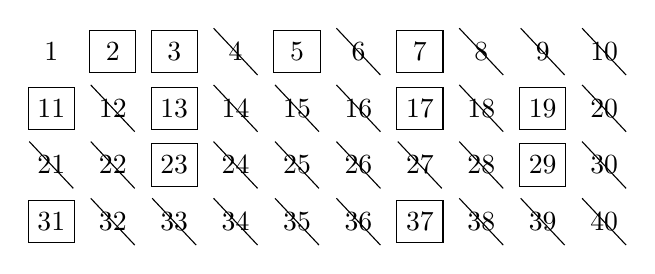
\begin{tikzpicture}[x=0.78cm,y=0.72cm]
    \foreach \n in {1,...,40} {
        \pgfmathtruncatemacro{\c}{mod(\n-1,10)}
        \pgfmathtruncatemacro{\r}{int((\n-1)/10)}
        \node[minimum width=1.35em,minimum height=1.25em,inner sep=1pt]
            (s\n) at (\c,-\r) {\(\n\)};
    }
    \foreach \p in {2,3,5,7,11,13,17,19,23,29,31,37} {
        \draw ([shift={(-1.4pt,1.2pt)}]s\p.north west)
              rectangle
              ([shift={(1.4pt,-1.2pt)}]s\p.south east);
    }
    \foreach \m in {4,6,8,9,10,12,14,15,16,18,20,21,22,24,25,26,27,28,30,32,33,34,35,36,38,39,40} {
        \draw ([shift={(-1pt,2pt)}]s\m.north west)
              --
              ([shift={(1pt,-2pt)}]s\m.south east);
    }
\end{tikzpicture}
\caption{Sieve of Eratosthenes on \(\{1,\ldots,40\}\). Primes are boxed and
composite numbers are struck out. The entry \(1\) is neither.}
\end{figure}

List a run of integers and strike out multiples of primes, and of prime
powers, in increasing order, keeping only prime powers that are at most
the smoothness bound \(B\). What survives is \(B\)-smooth.

\subsection{The quadratic sieve}
\label{sec:qs}

The quadratic sieve (Pomerance) turns the same idea into a factoring
algorithm. The goal is to find an integer \(a\) such that \(a^{2}\bmod N\)
is \(B\)-smooth.

Start from the polynomial \(F(t)=t^{2}-N\). List the values
\[
    F(a),\; F(a+1),\; \ldots,\; F(b),
\]
where \(a=\lfloor\sqrt{N}\rfloor+1\) and the right endpoint \(b\) is large
enough that the list contains about \(L(N)^{\sqrt{2}}\) entries. An entry
is \(B\)-smooth precisely when every prime dividing it is at most \(B\).

For an odd prime \(p\le B\), the congruence \(t^{2}-N\equiv 0\pmod{p}\)
has either no solution or two solutions modulo \(p\). If \(\alpha_{p}\) and
\(\beta_{p}\) are the two solutions, then every integer in either of the
arithmetic progressions
\[
    \alpha_{p}+p,\;\alpha_{p}+2p,\;\alpha_{p}+3p,\;\ldots
    \qquad\text{and}\qquad
    \beta_{p}+p,\;\beta_{p}+2p,\;\beta_{p}+3p,\;\ldots
\]
is likewise a solution. At each such argument, \(p\) divides \(F(t)\), so
the sieve can divide the whole progression by \(p\) (and by the prime
powers \(p^{e}\le B\)) in one pass.

% --- page 54 ---

\begin{example}[Sieving \(F(t)=t^{2}-221\)]
Let \(N=221\). Then \(\sqrt{N}\approx 14.9\), so the list begins at
\(t=15\):
\[
    F(t)=t^{2}-N,\qquad t=15,16,17,\ldots.
\]
Dividing by \(2\), \(4\), \(5\), and \(7\) along the progressions above
produces the following array. An arrow means that the entry is divisible
by the next prime power and is replaced by the quotient.

\begin{figure}[H]
\centering
\setlength{\tabcolsep}{5.5pt}
\renewcommand{\arraystretch}{1.18}
\begin{tabular}{l|cccccccc}
    & \(15\) & \(16\) & \(17\) & \(18\) & \(19\) & \(20\) & \(21\) & \(22\) \\
    \hline
    \(F(t)\)
        & \(4\) & \(35\) & \(68\) & \(103\) & \(140\) & \(179\) & \(220\) & \(263\) \\
        & \(\downarrow\) & & \(\downarrow\) & & \(\downarrow\) & & \(\downarrow\) & \\
    divide by \(2\)
        & \(2\) & & \(34\) & & \(70\) & & \(110\) & \\
        & \(\downarrow\) & & \(\downarrow\) & & \(\downarrow\) & & \(\downarrow\) & \\
    divide by \(4\)
        & \(1\) & & \(17\) & & \(35\) & & \(55\) & \\
        & & \(\downarrow\) & & & \(\downarrow\) & & \(\downarrow\) & \\
    divide by \(5\)
        & & \(7\) & & & \(7\) & & \(11\) & \\
        & & \(\downarrow\) & & & \(\downarrow\) & & & \\
    divide by \(7\)
        & & \(1\) & & & \(1\) & & & \\
\end{tabular}
\caption{Quadratic sieve for \(N=221\) on \(t=15,\ldots,22\). Blank cells
are not divisible by that prime power. A final entry \(1\) means that
\(F(t)\) factored completely over \(\{2,5,7\}\).}
\end{figure}

The prime \(p=3\) never occurs. Indeed
\[
    221\equiv 2\pmod{3},
\]
and \(2\) is not a square modulo \(3\), so \(t^{2}\equiv 221\pmod{3}\) has
no solution and the progression for \(p=3\) is empty.

\begingroup\samepage
Reading off the rows that reach \(1\), together with the two further
arguments \(t=21\) and \(t=23\) whose cofactor is the prime \(11\),
\begin{align*}
    15^{2}-N &= 2^{2},\\
    16^{2}-N &= 5\cdot 7,\\
    19^{2}-N &= 2^{2}\cdot 5\cdot 7,\\
    21^{2}-N &= 2^{2}\cdot 5\cdot 11,\\
    23^{2}-N &= 2^{2}\cdot 7\cdot 11.
\end{align*}
\endgroup
% FIX p.54: \(23^{2}-221=308=2^{2}\cdot 7\cdot 11\). A first reading of the
% exponent of \(2\) is ambiguous; the integer factorisation forces \(2^{2}\).
The second and third relations multiply to a square on both sides:
\[
    (5\cdot 7)\cdot(2^{2}\cdot 5\cdot 7)
    =(2\cdot 5\cdot 7)^{2},
\]
so
\[
    (16\cdot 19)^{2}\equiv(2\cdot 5\cdot 7)^{2}\pmod{N}.
\]
Set \(a=16\cdot 19=304\) and \(b=70\). Then \(a-b=234\), and
\[
    \gcdop(234,221)=13.
\]
Thus \(N=13\cdot 17\).
\end{example}

% --- page 55 ---

The same list contains a second dependency, and it is useless. Multiplying
the relations for \(t=16\), \(21\), and \(23\) gives exponents
\(2^{4}\cdot 5^{2}\cdot 7^{2}\cdot 11^{2}\), hence
\[
    (16\cdot 21\cdot 23)^{2}
    \equiv(2^{2}\cdot 5\cdot 7\cdot 11)^{2}\pmod{N}.
\]
Here \(a=16\cdot 21\cdot 23=7728\) and \(b=2^{2}\cdot 5\cdot 7\cdot 11=1540\), so
\begin{align*}
    \gcdop(a-b,N)&=\gcdop(6188,221)=221,\\
    \gcdop(a+b,N)&=\gcdop(9268,221)=1.
\end{align*}
Both greatest common divisors are trivial factors of \(N\).

\begin{remark}
Let \(p\) be an odd prime and let \(e\ge 1\). In the situation used by the
sieve, where \(p\) does not divide \(N\), the congruence
\[
    t^{2}\equiv N\pmod{p^{e}}
\]
has either no solution or exactly two solutions.
% FIX p.55: the notes omit the hypothesis that \(p\) does not divide \(N\).
% Without it the count of solutions can fail (for instance if \(p\) divides \(N\)).
\end{remark}

Concretely, before a prime \(p\) is used in the sieve one has to decide
whether \(N\) is a square modulo \(p\). For \(N=221\) and \(p=3\) it is not,
as above.

Quadratic residuosity is not only a sieving test. The distinction between
quadratic residues and quadratic non-residues can be used as the hidden
bit of a public-key encryption scheme, the Goldwasser--Micali cryptosystem.

If the plaintext were a bare bit \(m\in\{0,1\}\) and the encryption map
were deterministic, an eavesdropper would recognise \(m\) just by comparing
a ciphertext with the two possible encryptions. The way around this is to
pad the bit with randomness: replace \(m\) by a pair \((m,x)\) that is
sufficiently random, and encrypt the pair.

% --- page 56 ---

\section{The Goldwasser--Micali cryptosystem}
\label{sec:gm}

\paragraph{Key generation.}
Alice chooses two primes \(p\) and \(q\), and an integer \(a\) with
\[
    \Bigl(\frac{a}{p}\Bigr)=-1
    \qquad\text{and}\qquad
    \Bigl(\frac{a}{q}\Bigr)=-1.
\]
She publishes the modulus \(N=pq\) and the quadratic non-residue \(a\), and
she keeps the factorization \((p,q)\).

\paragraph{Encryption.}
Bob wants to send a bit \(m\in\{0,1\}\). He chooses an integer \(x\) with
\(1<x<N\) at random and sends
\[
    c\equiv
    \begin{cases}
        x^{2}\pmod{N} & \text{if }m=0,\\
        ax^{2}\pmod{N} & \text{if }m=1.
    \end{cases}
\]

\paragraph{Decryption.}
Alice receives \(c\) and computes the Legendre symbols
\(\bigl(\frac{c}{p}\bigr)\) and \(\bigl(\frac{c}{q}\bigr)\). For the symbol
modulo \(p\), and assuming \(\gcdop(x,N)=1\),
\[
    \Bigl(\frac{c}{p}\Bigr)
    =
    \begin{cases}
        \Bigl(\dfrac{x^{2}}{p}\Bigr)
            =\Bigl(\dfrac{x}{p}\Bigr)^{2}
            =1 & \text{if }m=0,\\[1.6em]
        \Bigl(\dfrac{ax^{2}}{p}\Bigr)
            =\Bigl(\dfrac{a}{p}\Bigr)\Bigl(\dfrac{x}{p}\Bigr)^{2}
            =-1 & \text{if }m=1.
    \end{cases}
\]
The same computation modulo \(q\) gives
\[
    \Bigl(\frac{c}{q}\Bigr)
    =
    \begin{cases}
        1 & \text{if }m=0,\\
        -1 & \text{if }m=1.
    \end{cases}
\]
Either symbol is therefore \((-1)^{m}\), and Alice recovers the bit.

\paragraph{What Eve sees.}
Eve knows \(N\), \(a\), and \(c\), and she can form the Jacobi symbol
\(\bigl(\frac{c}{N}\bigr)\). In both cases the value lies in \(\{1,0\}\):
\[
    \Bigl(\frac{c}{N}\Bigr)
    =
    \begin{cases}
        \Bigl(\dfrac{x^{2}}{N}\Bigr)
            =\Bigl(\dfrac{x}{N}\Bigr)^{2}
            \in\{1,0\} & \text{if }m=0,\\[1.6em]
        \Bigl(\dfrac{ax^{2}}{N}\Bigr)
            =\Bigl(\dfrac{x}{N}\Bigr)^{2}\Bigl(\dfrac{a}{pq}\Bigr)
            =\Bigl(\dfrac{x}{N}\Bigr)^{2}
            \underbrace{\Bigl(\dfrac{a}{p}\Bigr)\Bigl(\dfrac{a}{q}\Bigr)}_{=\,1}
            \in\{1,0\} & \text{if }m=1.
    \end{cases}
\]
The symbol equals \(1\) when \(\gcdop(x,N)=1\) and equals \(0\) when \(p\) or
\(q\) divides \(x\). It is never \(-1\), so it does not reveal the bit.
The factorization of \(N\) is what makes the two Legendre symbols available
to Alice.

% --- page 57 ---

\begin{remark}
The scheme as written is not practical: each ciphertext, a number modulo
\(N\), carries a single bit of message.
\end{remark}

\section{Index calculus}
\label{sec:index-calculus}

Index calculus is a subexponential algorithm for the discrete logarithm
problem in \(\units{p}\). Recall from Lecture~12 that the problem is: given a prime \(p\), a primitive
root \(g\) modulo \(p\), and a target \(h\in\units{p}\), find the integer
\(x\) with \(1\le x\le p-1\) and
\[
    g^{x}\equiv h\pmod{p}.
\]
That integer is \(x=\ind_{g}(h)\).

Instead of attacking \(h\) directly, first solve
\[
    g^{x}\equiv \ell\pmod{p}
\]
for every prime \(\ell\le B\), for a smoothness bound \(B\) still to be
chosen. The solutions are the factor-base logarithms \(\ind_{g}(\ell)\).

The individual logarithm is then a search for one further smooth value.
Compute \(hg^{k}\bmod p\) for \(k=1,2,3,\ldots\) until the residue is
\(B\)-smooth, say
\[
    hg^{k}
    \equiv\prod_{\ell\le B}\ell^{e_{\ell}}\pmod{p}.
\]
Taking \(\ind_{g}\) of both sides yields the linear congruence
\[
    \ind_{g}(h)+k
    \equiv\sum_{\ell\le B}e_{\ell}\,\ind_{g}(\ell)
    \pmod{p-1},
\]
and therefore
\[
    \ind_{g}(h)
    \equiv -k+\sum_{\ell\le B}e_{\ell}\,\ind_{g}(\ell)
    \pmod{p-1}.
\]

\lectureheading{Lecture 21 (30/10/26)}

% --- page 58 ---

The missing ingredient is the computation of \(\ind_{g}(\ell)\) for the
primes \(\ell\le B\). Draw exponents \(i\ge 1\) at random and set
\[
    g_{i}\equiv g^{i}\pmod{p}.
\]
Whenever \(g_{i}\) is \(B\)-smooth, write
\[
    g_{i}=\prod_{\ell\le B}\ell^{e_{\ell}(i)}
\]
in \(\Z\), up to the representative chosen modulo \(p\). Then
\[
    \ind_{g}(g_{i})
    \equiv\sum_{\ell\le B}e_{\ell}(i)\,\ind_{g}(\ell)
    \pmod{p-1},
\]
and since \(\ind_{g}(g_{i})\equiv i\pmod{p-1}\),
\[
    i\equiv\sum_{\ell\le B}e_{\ell}(i)\,\ind_{g}(\ell)
    \pmod{p-1}.
\]
Each smooth \(g_{i}\) is one linear equation in the unknowns
\(\ind_{g}(\ell)\), \(\ell\le B\). Enough such equations determine those
unknowns.

The modulus of the system is \(p-1\). By the Chinese Remainder Theorem it
is enough to solve the system modulo \(q^{\alpha}\) for each prime power
\(q^{\alpha}\) in the factorization of \(p-1\): solve first modulo \(q\),
then lift the solution to \(q^{\alpha}\).

The smooth-number count of the previous lecture applies with \(x=p\).
If the factor base is cut at
\[
    B=L(p)^{1/\sqrt{2}},
\]
one expects to test about \(L(p)^{\sqrt{2}}\) exponents \(i\) before
enough relations have been found.

As in the quadratic sieve, the relations should be collected by a sieve.
Rather than factoring each \(g^{i}\bmod p\) from scratch, list the
candidates and divide by primes and prime powers wherever the
corresponding congruence permits it.

% --- page 59 ---

\begin{example}[A small index calculus]
\label{ex:index}
Let \(p=232487\), and take \(g=229401\) and \(h=171020\). The problem is
to solve \(g^{x}\equiv h\pmod{p}\).

Take the smoothness bound \(B=7\), so the factor base is
\(\{2,3,5,7\}\). Four smooth relations are
\begin{align*}
    g^{482}&\equiv 2^{5}\cdot 3^{2}\cdot 7^{3}\pmod{p},\\
    g^{600}&\equiv 2^{2}\cdot 3^{9}\pmod{p},\\
    g^{876}&\equiv 2^{9}\cdot 3^{4}\pmod{p},\\
    g^{948}&\equiv 2^{6}\cdot 5^{2}\pmod{p}.
\end{align*}
Write \(x_{i}=\ind_{g}(i)\) for \(i\in\{2,3,5,7\}\). The relations become
the linear system
\begin{align*}
    482&\equiv 5x_{2}+2x_{3}+3x_{7},\\
    600&\equiv 2x_{2}+9x_{3},\\
    876&\equiv 9x_{2}+4x_{3},\\
    948&\equiv 6x_{2}+2x_{5},
\end{align*}
which the notes record modulo \((p-1)/2\). Each congruence is an equality
of indices, so it holds modulo \(p-1\) as well. The modulus factors as
\(p-1=232486=2\cdot 116243\). Reducing modulo \(2\) gives
\begin{align*}
    x_{2}+x_{7}&\equiv 0\pmod{2},\\
    x_{3}&\equiv 0\pmod{2},\\
    x_{2}&\equiv 0\pmod{2},
\end{align*}
while the last equation is \(0\equiv 0\pmod{2}\) and does not constrain
\(x_{5}\). Therefore
\[
    x_{2}\equiv x_{3}\equiv x_{7}\equiv 0\pmod{2},
\]
and \(x_{5}\) may be either even or odd.

Solving the original system modulo \((p-1)/2=116243\) produces one
solution class
\begin{align*}
    x_{2}&\equiv 38292,\\
    x_{3}&\equiv 30305,\\
    x_{5}&\equiv 1841,\\
    x_{7}&\equiv 71128,
\end{align*}
all modulo \((p-1)/2\).

% --- page 60 ---
The parity conditions select the lifts of \(x_{2}\), \(x_{3}\), and
\(x_{7}\). The representatives \(38292\) and \(71128\) are already even,
while \(30305\) is odd, so
\begin{align*}
    x_{2}&\equiv 38292,\\
    x_{3}&\equiv 30305+116243=146548,\\
    x_{7}&\equiv 71128,
\end{align*}
modulo \(p-1\). For \(x_{5}\) the coefficient in the system is even, so
both lifts satisfy the congruences. The power
\[
    g^{1841}\equiv 5\pmod{p}
\]
selects \(x_{5}\equiv 1841\pmod{p-1}\).
% The notes cross out a side product \(117\times 84\) between
% \(x_{5}\equiv 1841\) and \(5=g^{1841}\pmod{p}\). It is not used.

A further smooth multiple of the target is
\[
    g^{166}\cdot h\equiv 2^{7}\cdot 3^{2}\cdot 5^{2}\cdot 7\pmod{p}.
\]
Taking indices,
\[
    166+\ind_{g}(h)
    \equiv 7x_{2}+2x_{3}+2x_{5}+x_{7}
    \pmod{p-1}.
\]
The right-hand side evaluates to
\begin{align*}
    7\cdot 38292+2\cdot 146548+2\cdot 1841+71128
    &=635950\\
    &=2(p-1)+170978,
\end{align*}
so
\[
    \ind_{g}(h)
    \equiv 170978-166
    =170812\pmod{p-1}.
\]
% The notes record the result \(170812\) without the intermediate sum.
% The arithmetic above is that skipped evaluation.
Thus \(g^{170812}\equiv h\pmod{p}\).
\end{example}

Index calculus solves the discrete logarithm problem in \(\units{p}\) in
subexponential time.

\section{Elliptic Curves}
\label{sec:ec-warmup}

Discrete logarithms on elliptic curves, by contrast,
require exponential time with the algorithms available for a general curve.

\subsection{Warm-up: rational points on the circle}

Consider the circle \(C\colon x^{2}+y^{2}=1\).

\begin{figure}[H]
\centering
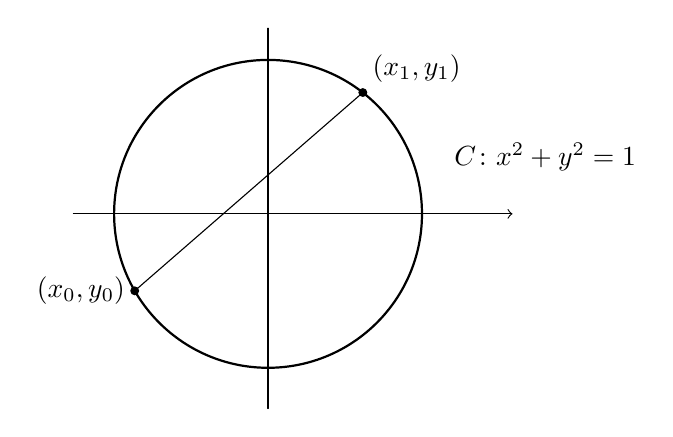
\begin{tikzpicture}[scale=1.15,line cap=round]
    \draw[thick] (0,0) circle (1.7);
    \draw[->] (-2.15,0) -- (2.7,0);
    \draw (0,-2.15) -- (0,2.05);
    \coordinate (P0) at (210:1.7);
    \coordinate (P1) at (52:1.7);
    \draw (P0) -- (P1);
    \fill (P0) circle (1.4pt);
    \fill (P1) circle (1.4pt);
    \node[left] at (P0) {\((x_{0},y_{0})\)};
    \node[above right] at (P1) {\((x_{1},y_{1})\)};
    \node[anchor=west] at (18:2.05) {\(C\colon x^{2}+y^{2}=1\)};
\end{tikzpicture}
\caption{The circle \(C\colon x^{2}+y^{2}=1\), with a chord through two of
its points.}
\end{figure}

The aim is to study the points of this curve, then to study them by means
of a parameter, and in particular to study the rational points by means of
a rational parameter.

% --- page 61 ---

A point is rational when it lies in \(\mathbb{Q}^{2}\). The integer points
on \(C\) are
\[
    \bigl\{(\pm 1,0),\,(0,\pm 1)\bigr\}.
\]
There are many further rational points, for instance
\[
    \Bigl(\frac{3}{5},\frac{4}{5}\Bigr),
    \qquad
    \Bigl(\frac{5}{13},\frac{12}{13}\Bigr),
    \qquad\ldots,
\]
coming from primitive Pythagorean triples.

\begin{claim}
Let \((x_{0},y_{0})\) and \((x_{1},y_{1})\) be rational points of \(C\).
The line through them has rational slope.
\end{claim}

Conversely, start with one rational point \((x_{0},y_{0})\) and a rational
slope \(t\). The line of slope \(t\) through \((x_{0},y_{0})\) meets \(C\)
again at a point \((x_{1},y_{1})\). That second point is rational: already
\(x_{1}\in\mathbb{Q}\), or equivalently \(y_{1}\in\mathbb{Q}\), and
therefore \((x_{1},y_{1})\in\mathbb{Q}^{2}\).

Take the base point to be \((x_{0},y_{0})=(-1,0)\). The line of slope \(t\)
through this point is \(y=t(x+1)\). It meets the tangent line \(x=1\) at
the point \((1,2t)\), which is the picture used to solve for the second
intersection with the circle.

\begin{figure}[H]
\centering
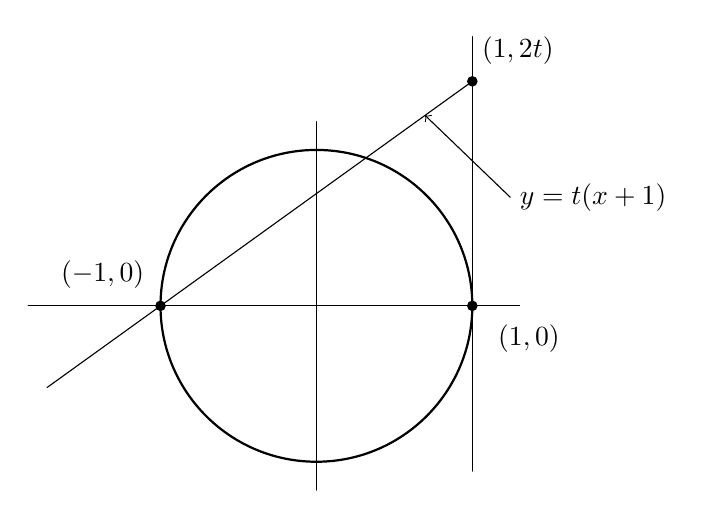
\begin{tikzpicture}[scale=1.2,line cap=round]
    \draw[thick] (0,0) circle (1.65);
    \draw (-3.05,0) -- (2.15,0);
    \draw (0,-1.95) -- (0,1.95);
    % unit circle scaled by 1.65; the line x=1 is tangent at (1,0)
    \draw (1.65,-1.75) -- (1.65,2.85);
    % y=t(x+1) with t=0.72; picture height of (1,2t) is 2*0.72*1.65
    \draw (-2.85,-0.864) -- (1.65,2.376);
    \fill (-1.65,0) circle (1.6pt);
    \node[above left] at (-1.72,0.08) {\((-1,0)\)};
    \fill (1.65,0) circle (1.6pt);
    \node[anchor=north west] at (1.82,-0.10) {\((1,0)\)};
    \fill (1.65,2.376) circle (1.6pt);
    \node[above right] at (1.65,2.45) {\((1,2t)\)};
    \node[anchor=west] (eq) at (2.05,1.15) {\(y=t(x+1)\)};
    \draw[->] (eq.west) -- (1.15,2.016);
\end{tikzpicture}
\caption{The line \(y=t(x+1)\) through \((-1,0)\). It meets the tangent
line \(x=1\) at \((1,2t)\).}
\end{figure}

% CONTINUES: rational points on the circle $x^2+y^2=1$, via lines of rational slope through $(-1,0)$.
% --- page 62 ---

The line through $(-1,0)$ of slope $t$ is $y=t(x+1)$. Substituting into the circle gives
\[
    \bigl(t(x+1)\bigr)^2+x^2=1,
\]
which expands to the quadratic
\[
    x^2(1+t^2)+2t^2 x+(t^2-1)=0.
\]
One root is the known intersection $x=-1$. Factoring,
\[
    (x+1)\bigl((1+t^2)x-(1-t^2)\bigr)
    =x^2(1+t^2)+2t^2 x+(t^2-1),
\]
so the other root is
\[
    x=\frac{1-t^2}{1+t^2}.
\]
The corresponding $y$-coordinate is
\[
    y=t(x+1)=t\left(\frac{1-t^2}{1+t^2}+1\right)
    =\frac{2t}{1+t^2}.
\]
Thus every rational slope produces a rational point, and every rational point other than $(-1,0)$ arises this way:
\[
    \left\{
        \left(\frac{1-t^2}{1+t^2},\,\frac{2t}{1+t^2}\right)
        : t\in\mathbb{Q}
    \right\}
    \cup\{(-1,0)\}.
\]
Sending $t\to\infty$ (the vertical line through $(-1,0)$) returns the missing point: the two coordinates tend to $-1$ and $0$.

\subsection{The group law}

The name is historical. Arc lengths of ellipses lead to elliptic integrals, and elliptic integrals lead to the curves below.

\begin{keybox}
\begin{definition}[Elliptic curve]
For us, an elliptic curve is an equation
\[
    y^2=x^3+ax+b,
\]
where $a,b\in\R$ satisfy $4a^3+27b^2\neq 0$. The condition ensures that the cubic has no repeated root, so the curve is nonsingular.
\end{definition}
\end{keybox}

% --- page 63 ---

Over $\R$ the real locus has one of the two shapes in Figure~\ref{fig:ec-real}, according to the number of real roots of the cubic. A cross marks a root.

\begin{figure}[H]
\centering
\begin{tikzpicture}[x=0.78cm,y=0.78cm,line cap=round,line join=round]
    % one real component: y^2 = x^3 - x + 1, root about -1.325
    \begin{scope}
        \draw[->] (-2.15,0) -- (2.15,0);
        \draw (0,-1.85) -- (0,1.85);
        \draw[domain=-1.32472:1.85,samples=240,smooth] plot (\x,{sqrt(max(0,\x*\x*\x-\x+1))});
        \draw[domain=-1.32472:1.85,samples=240,smooth] plot (\x,{-sqrt(max(0,\x*\x*\x-\x+1))});
        \node[fill=white,inner sep=1pt] at (-1.325,0) {$\times$};
    \end{scope}
    % two components: y^2 = x^3 - 4x, roots -2,0,2
    \begin{scope}[xshift=6.6cm]
        \draw[->] (-2.7,0) -- (3.55,0);
        \draw (1,-1.85) -- (1,1.85);
        \draw[domain=-2:0,samples=240,smooth] plot (\x,{sqrt(max(0,\x*\x*\x-4*\x))});
        \draw[domain=-2:0,samples=240,smooth] plot (\x,{-sqrt(max(0,\x*\x*\x-4*\x))});
        \draw[domain=2:2.85,samples=240,smooth] plot (\x,{sqrt(max(0,\x*\x*\x-4*\x))});
        \draw[domain=2:2.85,samples=240,smooth] plot (\x,{-sqrt(max(0,\x*\x*\x-4*\x))});
        \node[fill=white,inner sep=1pt] at (-2,0) {$\times$};
        \node[fill=white,inner sep=1pt] at (0,0) {$\times$};
        \node[fill=white,inner sep=1pt] at (2,0) {$\times$};
    \end{scope}
\end{tikzpicture}
\caption{Real locus of a short Weierstrass equation. Left: $y^2=x^3-x+1$, one real root. Right: $y^2=x^3-4x$, three real roots, drawn as an oval and an unbounded component, with a vertical line in the gap between them.}
\label{fig:ec-real}
\end{figure}

This shape of equation is called the \emph{Weierstrass form}. It is available whenever $\operatorname{char} K\neq 2,3$. In the remaining characteristics one uses
\begin{align*}
    \operatorname{char} K=2:
    &\quad
    \begin{cases}
        y^2+cy=x^3+ax+b,\\
        y^2+xy=x^3+ax^2+b,
    \end{cases}\\[0.4em]
    \operatorname{char} K=3:
    &\quad
    y^2=x^3+ax^2+bx+c.
\end{align*}
The general Weierstrass equation, over any field, is
\[
    y^2+a_1 xy+a_3 y=x^3+a_2 x^2+a_4 x+a_6.
\]

An elliptic curve comes with a point at infinity. That extra point is what makes it possible to put an abelian group structure on the curve.

Adding two points by adding coordinates does not work. If $(x_1,y_1)$ and $(x_2,y_2)$ lie on $E$, the pair $(x_1+x_2,\,y_1+y_2)$ need not.

% --- page 64 ---

A second attempt uses the geometry of a line. Let $P$ and $Q$ be points of $E$, and let the line through them meet $E$ again at $R$, as in Figure~\ref{fig:ec-naive}.

\begin{figure}[H]
\centering
\begin{tikzpicture}[x=0.72cm,y=0.72cm,line cap=round,line join=round]
    \draw[->] (-2.7,0) -- (4.15,0);
    % y-axis in the gap (0,2); x=0 is a root, with a vertical tangent
    \draw[gray!55] (0,-4.3) -- (0,4.3);
    \draw[domain=-2:0,samples=240,smooth] plot (\x,{sqrt(max(0,\x*\x*\x-4*\x))});
    \draw[domain=-2:0,samples=240,smooth] plot (\x,{-sqrt(max(0,\x*\x*\x-4*\x))});
    \draw[domain=2:3.30,samples=240,smooth] plot (\x,{sqrt(max(0,\x*\x*\x-4*\x))});
    \draw[domain=2:3.30,samples=240,smooth] plot (\x,{-sqrt(max(0,\x*\x*\x-4*\x))});
    % P, Q, R lie on y^2=x^3-4x; chord y+0.397=0.881(x+1.98) ends on R
    \coordinate (P) at (-1.98,-0.397);
    \coordinate (Q) at (-0.30,1.083);
    \coordinate (R) at (3.056,4.040);
    \draw (-2.32,-0.696) -- (R);
    \draw[->] (-0.72,0.713) -- (-0.48,0.924);
    \fill (P) circle (1.6pt);
    \node[anchor=north east] at (-2.08,-0.58) {$P$};
    \fill (Q) circle (1.6pt);
    \node[above=3pt] at (Q) {$Q$};
    \fill (R) circle (1.6pt);
    \node[above left=1pt] at (R) {$R$};
\end{tikzpicture}
\caption{The chord through $P$ and $Q$ on $y^2=x^3-4x$ meets the curve again at $R$. Declaring $P+Q=R$ does not give a group law.}
\label{fig:ec-naive}
\end{figure}

\begin{remark}
Taking $P+Q$ to be this third point $R$ fails. The three intersection points are symmetric, so the same rule would also require $Q+R=P$ and $P+R=Q$, and those identities do not hold. The proposal collapses further to $2P=2Q=2R=\mathcal{O}_E$, i.e.\ every point would have order dividing $2$. The notes mark the attempt with $(\times)$; it also fails.
\end{remark}

The law that does work reflects the third intersection across the $x$-axis. Draw the line through $P$ and $Q$, let $R$ be its third meeting with $E$, and let $R'$ be the reflection of $R$ in the $x$-axis (Figure~\ref{fig:ec-sum}). Define
\[
    P+Q=R'.
\]

\begin{figure}[H]
\centering
\begin{tikzpicture}[x=0.78cm,y=0.78cm,line cap=round,line join=round]
    \draw[->] (-2.55,0) -- (4.05,0);
    % y-axis in the gap (0,2); x=0 is a root, with a vertical tangent
    \draw[gray!55] (0,-3.25) -- (0,3.15);
    \draw[domain=-2:0,samples=240,smooth] plot (\x,{sqrt(max(0,\x*\x*\x-4*\x))});
    \draw[domain=-2:0,samples=240,smooth] plot (\x,{-sqrt(max(0,\x*\x*\x-4*\x))});
    \draw[domain=2:3.25,samples=240,smooth] plot (\x,{sqrt(max(0,\x*\x*\x-4*\x))});
    \draw[domain=2:3.25,samples=240,smooth] plot (\x,{-sqrt(max(0,\x*\x*\x-4*\x))});
    % P, Q, R on y^2=x^3-4x; R' is the reflection of R
    \coordinate (P) at (-1.800,-1.170);
    \coordinate (Q) at (-0.040,0.400);
    \coordinate (R) at (2.635,2.786);
    \coordinate (Rp) at (2.635,-2.786);
    \draw (-2.15,-1.482) -- (R);
    \draw[dashed] (R) -- (Rp);
    \fill (P) circle (1.6pt);
    \node[anchor=north] at (-1.80,-1.32) {$P$};
    \fill (Q) circle (1.6pt);
    \node[anchor=east] at (-0.28,0.72) {$Q$};
    \fill (R) circle (1.6pt);
    \node[anchor=south west] at (2.78,2.90) {$R$};
    \fill (Rp) circle (1.6pt);
    \node[anchor=west] at (2.95,-2.55) {$R'=P+Q$};
\end{tikzpicture}
\caption{Chord through $P$ and $Q$ on $y^2=x^3-4x$, meeting the curve again at $R$. The dashed segment reflects $R$ across the $x$-axis to $R'$, and the sum is $P+Q=R'$.}
\label{fig:ec-sum}
\end{figure}

\par
\ifdim\dimexpr\pagegoal-\pagetotal<5\baselineskip
  \newpage
\fi
\begin{example}[Adding two distinct points]
\label{ex:pq-sum}
Take $y^2=x^3-15x+18$, with $P=(7,16)$ and $Q=(1,2)$. Both points lie on the curve:
\[
    16^2=256=7^3-15\cdot 7+18,
    \qquad
    2^2=4=1^3-15\cdot 1+18.
\]
The slope of the chord is
\[
    \frac{16-2}{7-1}=\frac{14}{6}=\frac{7}{3},
\]
so the line is
\[
    y-2=\frac{7}{3}(x-1),
    \qquad
    y=\frac{7}{3}x-\frac{1}{3}.
\]
Substitute into the curve:
\[
    \left(\frac{7}{3}x-\frac{1}{3}\right)^2=x^3-15x+18.
\]
Clearing the denominator $9$,
\begin{align*}
    (7x-1)^2&=9x^3-135x+162,\\
    49x^2-14x+1&=9x^3-135x+162,\\
    0&=9x^3-49x^2-121x+161.
\end{align*}
Dividing by $9$ gives the monic cubic whose roots are the $x$-coordinates of the three intersections:
\begin{equation}
    x^3-\frac{49}{9}x^2-\frac{121}{9}x+\frac{161}{9}=0.
    \label{eq:pq-cubic}
\end{equation}
% --- page 65 ---
The roots include $x=7$ and $x=1$. If $\lambda$ is the third, then
\[
    \lambda+1+7=\frac{49}{9},
    \qquad
    \lambda=\frac{49}{9}-8=\frac{49-72}{9}=-\frac{23}{9}.
\]
% FIX p.65: the notes write this reduction as $(49-8)/7=-23/9$.
% The sum of roots of \eqref{eq:pq-cubic} is $49/9$, so $\lambda=49/9-8=-23/9$.
% The value $-23/9$ written underneath is the correct root; $(49-8)/7=41/7$ is not.
The line at this abscissa has
\begin{align*}
    y
    &=\frac{7}{3}\left(-\frac{23}{9}\right)-\frac{1}{3}
     =\frac{-161-9}{27}
     =-\frac{170}{27}.
\end{align*}
% FIX p.65: the notes record the intersection ordinate as $-170/9$ and the sum as $(-23/9,\,170/9)$.
% The line is $y=(7x-1)/3$, so $y=(-170/9)/3=-170/27$.
Reflecting across the $x$-axis,
\[
    P+Q=\left(-\frac{23}{9},\,\frac{170}{27}\right).
\]
\end{example}

\lectureheading{Lecture 22 (03/11/26)}

To double a point, replace the chord by the tangent. Let the tangent line to $E$ at $P$ meet $E$ again at $R$. Then $P+P$ is the reflection of $R$ across the $x$-axis.

\begin{example}[Doubling]
Continue with $y^2=x^3-15x+18$ and $P=(7,16)$. Differentiating implicitly,
\[
    2yy'=3x^2-15,
    \qquad
    y'=\frac{3x^2-15}{2y}.
\]
The slope of the tangent at $P$ is
\[
    \frac{3\cdot 7^2-15}{2\cdot 16}
    =\frac{3\cdot 49-15}{32}
    =\frac{132}{32}
    =\frac{33}{8}.
\]
The tangent line is
\[
    y=\frac{33}{8}(x-7)+16
    =\frac{33}{8}x-\frac{103}{8}.
\]
% --- page 66 ---
For the third intersection, substitute into the curve:
\[
    \left(\frac{33x-103}{8}\right)^2=x^3-15x+18.
\]
Expanding $(33x-103)^2=1089x^2-6798x+10609$ and $64(x^3-15x+18)=64x^3-960x+1152$, rearranging yields
\[
    64x^3-1089x^2+5838x-9457=0,
\]
or
\[
    x^3-\frac{1089}{64}x^2+\frac{2919}{32}x-\frac{9457}{64}=0.
\]
The point $P$ is a point of tangency, so $x=7$ is a double root. The third root therefore satisfies
\[
    7+7+x=\frac{1089}{64},
    \qquad
    x=\frac{1089}{64}-14
     =\frac{1089-896}{64}
     =\frac{193}{64}.
\]
% FIX p.66: the third root is written as $(1089-14)/64=193/64$.
% That quotient is $1075/64$. The sum of roots gives $1089/64-14=193/64$, which is the value used below.
The tangent at this abscissa has
\begin{align*}
    y
    &=\frac{33}{8}\cdot\frac{193}{64}-\frac{103}{8}
     =\frac{33\cdot 193-103\cdot 64}{512}
     =\frac{6369-6592}{512}
     =-\frac{223}{512}.
\end{align*}
Reflecting across the $x$-axis,
\[
    2P=P+P=\left(\frac{193}{64},\,\frac{223}{512}\right).
\]
\end{example}

\paragraph{Inverses and the identity.}
The same rule has to add a point to its reflection $(x,-y)$, and a point to the point at infinity.

The line through $(x,y)$ and $(x,-y)$ is vertical, so it meets $E$ at no further affine point. Declare that the point at infinity lies on every vertical line, and write $\mathcal{O}$ for that point. The vertical line then meets $E$ at $(x,y)$, $(x,-y)$, and $\mathcal{O}$, and the group law gives
\[
    (x,y)+(x,-y)=\mathcal{O}.
\]
In the other direction, the vertical line through $P=(x,y)$ meets $E$ again at $P'=(x,-y)$. Reflecting $P'$ across the $x$-axis returns $P$, so
\[
    P+\mathcal{O}=P.
\]

% --- page 67 ---

Thus $P+P'=\mathcal{O}$ with $P'=(x,-y)$. The point $(x,-y)$ is the inverse of $P$, written $-P$.

\begin{keybox}
\begin{theorem}[Group law]
\label{thm:group-law}
Let $E$ be an elliptic curve as above. The addition just defined has the following properties.
\begin{enumerate}[leftmargin=1.6em,label=\textup{(\arabic*)}]
    \item $P+\mathcal{O}=\mathcal{O}+P=P$.
    \item $P+(-P)=\mathcal{O}$.
    \item $P+Q=Q+P$.
    \item $(P+Q)+R=P+(Q+R)$.
\end{enumerate}
Associativity needs a separate rigorous proof; it is not checked from the pictures.
\end{theorem}
\end{keybox}

\subsection{The addition algorithm}

Let $E\colon y^2=x^3+Ax+B$, and let $P_1,P_2$ be points of $E$.
\begin{enumerate}[leftmargin=1.6em,label=\textup{(\arabic*)}]
    \item If $P_1=\mathcal{O}$, then $P_1+P_2=P_2$. If $P_2=\mathcal{O}$, then $P_1+P_2=P_1$.
    \item Otherwise write $P_1=(x_1,y_1)$ and $P_2=(x_2,y_2)$. If $x_1=x_2$ and $y_1=-y_2$, then $P_1+P_2=\mathcal{O}$.
    \item Otherwise define $\lambda$, $x_3$, and $y_3$ as follows, and set $P_1+P_2=(x_3,y_3)$.
\end{enumerate}

% --- page 68 ---

In case~(3),
\begin{equation}
    \lambda=
    \begin{cases}
        \dfrac{y_2-y_1}{x_2-x_1} & \text{if }P_1\neq P_2,\\[1.1em]
        \dfrac{3x_1^2+A}{2y_1} & \text{if }P_1=P_2,
    \end{cases}
    \label{eq:lambda}
\end{equation}
and
\begin{align}
    x_3&=\lambda^2-x_1-x_2, \label{eq:x3}\\
    y_3&=\lambda(x_1-x_3)-y_1. \label{eq:y3}
\end{align}
% FIX p.68: the formula line writes $y_3=\lambda(x_1-x_3)+y_1$.
% The proof just below derives the minus sign, which is the group law.
Then $P_1+P_2=(x_3,y_3)$.

\begin{proof}
In case~(3), $\lambda$ is the slope of the line through $P_1$ and $P_2$ (the tangent line, when the points coincide). That line is
\[
    y=\lambda x+\nu,
    \qquad
    \nu=y_1-\lambda x_1.
\]
Substitute into the curve:
\begin{align*}
    (\lambda x+\nu)^2&=x^3+Ax+B,\\
    x^3-\lambda^2 x^2+(A-2\lambda\nu)x+(B-\nu^2)&=0.
\end{align*}
The three roots are the abscissae of the intersections, so
\[
    \lambda^2=x_1+x_2+x_3,
    \qquad
    x_3=\lambda^2-x_1-x_2.
\]
The third intersection has ordinate $\lambda x_3+\nu$. Reflecting it across the $x$-axis gives the sum:
\begin{align*}
    y_3
    &=-(\lambda x_3+\nu)
     =-\lambda x_3-\nu
     =-\lambda x_3-(y_1-\lambda x_1)
     =\lambda(x_1-x_3)-y_1.
\end{align*}
\end{proof}

With this addition, the points of an elliptic curve form a group. The identity is the point at infinity $\mathcal{O}$.

\paragraph{Integer points.}
How many points with integer coordinates does $E$ have? For $A,B\in\Z$, Siegel's theorem says there are only finitely many integer points. Baker's method gives a bound on the number of those points.

% --- page 69 ---

\subsection{Rational points}

The rational points are much more structured than a finite set.

\begin{theorem}[Mordell--Weil]
The group $E(\mathbb{Q})$ of rational points, including $\mathcal{O}$, is a finitely generated abelian group:
\[
    E(\mathbb{Q})\;\cong\; G\times \Z^{r}.
\]
Here $G$ is a finite abelian group and the integer $r\geq 0$ is the \emph{rank} of the elliptic curve.
\end{theorem}

The rank is the quantity one most wants to understand for an elliptic curve over $\mathbb{Q}$. Bhargava's theorem says that a positive proportion of elliptic curves over $\mathbb{Q}$ have rank $0$, and a positive proportion have rank $1$.

If $r=0$, then $E(\mathbb{Q})$ itself is a finite abelian group. Mazur's theorem lists $15$ explicit possibilities for $G$. Those groups are too small to use for cryptography.

The Lutz--Nagell theorem says that, on the model $y^2=x^3+Ax+B$ with $A,B\in\Z$, every torsion point is an integer point.
% FIX p.69: the notes write ``Lutz-Nagelli''; the result is the Lutz--Nagell theorem.

\subsection{Elliptic curves over finite fields}

Now take an odd prime $p$, and an equation
\[
    y^2=x^3+Ax+B
    \qquad\text{with}\qquad
    4A^3+27B^2\not\equiv 0\pmod{p}.
\]
% --- page 70 ---
The set of solutions in $\Fp\times\Fp$, together with the point $\mathcal{O}$ at infinity, is a group under the same addition law. For each fixed $x$ one has to solve $y^2=x^3+Ax+B$ in $\Fp$.

\begin{example}[A curve over $\mathbb{F}_{13}$]
\label{ex:f13}
Let $E\colon y^2=x^3+3x+8$ over $\mathbb{F}_{13}$. The group is
\begin{align*}
    E(\mathbb{F}_{13})
    =\{&
        \mathcal{O},\;
        (1,5),\;(1,8),\;
        (2,3),\;(2,10),\\
        &(9,6),\;(9,7),\;
        (12,2),\;(12,11)
    \}.
\end{align*}
The same chord-and-tangent formulae work in $\Fp$. The notes ask whether these points carry a group structure; the answer is that one mimics the same addition law. Take $P=(9,7)$ and $Q=(1,8)$. Then
\[
    \lambda
    =\frac{8-7}{1-9}
    =\frac{1}{-8}.
\]
Modulo $13$ one has $-8\equiv 5$, and $5\cdot 8=40\equiv 1$, so $5^{-1}\equiv 8$ and $\lambda\equiv 8$. Then
\begin{align*}
    x_3
    &=\lambda^2-x_1-x_2
     =8^2-9-1
     =64-10
     =54
     \equiv 2\pmod{13},
\end{align*}
since $54-4\cdot 13=2$, and
\begin{align*}
    y_3
    &=\lambda(x_1-x_3)-y_1
     =8(9-2)-7
     =8\cdot 7-7
     =49
     \equiv 10\pmod{13},
\end{align*}
since $49-3\cdot 13=10$. (Equivalently $8\cdot 7-7=7\cdot 7=49$.) Therefore
\[
    P+Q=(2,10),
\]
which is one of the points listed above.
% FIX p.70: a sign in the handwritten line $8^2-9-1=64+10=54$ does not match $64-10=54$. The value $54\equiv 2$ used for $x_3$ is the correct one.
\end{example}

% --- page 71 ---

Doubling the same point $P=(9,7)$,
\begin{align*}
    \lambda
    &=\frac{3x_1^2+A}{2y_1}
     =\frac{3\cdot 9^2+3}{2\cdot 7}
     =\frac{246}{14}.
\end{align*}
Here $246=19\cdot 13-1\equiv -1\pmod{13}$ and $14\equiv 1\pmod{13}$, so $\lambda\equiv -1$. Then
\begin{align*}
    x_3
    &=\lambda^2-x_1-x_2
     =1-9-9
     =-17
     \equiv 9\pmod{13},\\
    y_3
    &=\lambda(x_1-x_3)-y_1
     =-1(9-9)-7
     =-7
     \equiv 6\pmod{13}.
\end{align*}
Hence $2P=(9,6)$.

\paragraph{The size of $E(\Fp)$.}
There are $p$ choices for $x$, and each gives at most two choices for $y$. Counting $\mathcal{O}$ as well,
\[
    \bigl|E(\Fp)\bigr|\leq 2p+1.
\]
About half of the values of $x$ make $x^3+Ax+B$ a quadratic residue, and about half make it a quadratic non-residue. The residue case contributes two points and the non-residue case contributes none, so one expects about $p$ affine points. Together with $\mathcal{O}$,
\[
    \bigl|E(\Fp)\bigr|\;\approx\; p+1.
\]
% FIX p.71: the notes equate $(p\cdot 2+1)/2$ with $p+1$.
% That quotient is $p+1/2$. The count intended by the residue heuristic is $(p/2)\cdot 2+1=p+1$.

\begin{keybox}
\begin{theorem}[Hasse bound]
\[
    \bigl|E(\Fp)\bigr|=(p+1)-t_p
    \qquad\text{with}\qquad
    |t_p|\leq 2\sqrt{p}.
\]
The bound is tight.
\end{theorem}
\end{keybox}
% FIX p.71: the notes spell the name ``Haase''; the bound is Hasse's.

% --- page 72 ---

The integer $t_p=(p+1)-\bigl|E(\Fp)\bigr|$ is called the \emph{trace of Frobenius}.
% FIX p.72: the notes write $t_p=\bigl|E(\Fp)\bigr|-(p+1)$, the negative of the trace appearing in the Hasse formula $|E(\Fp)|=(p+1)-t_p$ on the previous page.

\subsection{The elliptic-curve discrete logarithm}

\begin{keybox}
\begin{definition}[EC-DLP]
Let $E$ be an elliptic curve over $\Fp$, and let $P,Q\in E(\Fp)$. The elliptic-curve discrete logarithm problem asks for an integer $n$ such that
\[
    nP=Q,
\]
that is,
\[
    \underbrace{P+P+\cdots+P}_{n\text{ times}}=Q.
\]
The integer $n$ is called the discrete logarithm of $Q$ with respect to $P$, written $\log_P(Q)$. This is the additive form of the index $\ind$ of Lecture~12.
\end{definition}
\end{keybox}

\begin{remark}
As for the general discrete logarithm in Lecture~12, the equation $nP=Q$ can be solved if and only if $Q$ lies in the cyclic subgroup $\langle P\rangle$.
% FIX p.72: the notes spell ``solved'' as ``sowed''.
The solution is not unique: it is determined only modulo the order of $P$.
\end{remark}

\begin{example}[A curve over $\mathbb{F}_{73}$]
Let $y^2=x^3+8x+7$ over $\mathbb{F}_{73}$, and set
\begin{align*}
    P&=(32,53),\\
    Q&=(39,17)=11P,\\
    R&=(35,47)=37P.
\end{align*}
The order of $P$ is $41$. Since $11+37=48\equiv 7\pmod{41}$,
\[
    Q+R=11P+37P=48P=7P=(37,41).
\]
\end{example}

Alice, in the protocols built on this group, needs to compute $nP$. Adding $P$ to itself one step at a time produces the sequence $P,\,2P,\,3P,\,4P,\,\ldots$, which takes $n$ additions.

% --- page 73 ---

\paragraph{Double-and-add.}
Write the binary expansion
\[
    n=n_0+n_1\cdot 2+\cdots+n_r\cdot 2^r,
    \qquad
    n_i\in\{0,1\},
    \quad n_r=1.
\]
Compute the successive doubles
\[
    Q_0=P,
    \quad
    Q_1=2Q_0,
    \quad
    Q_2=2Q_1,
    \quad
    \ldots,
    \quad
    Q_r=2Q_{r-1}.
\]
Then $Q_i=2^i P$, and
\[
    nP=\sum_{i=0}^{r} n_i Q_i.
\]
Building the $Q_i$ costs $r$ doublings, and summing the terms with $n_i=1$ costs at most $r$ further additions, so $nP$ is obtained in at most $2r$ group operations. Because $n_r=1$,
\[
    2^r\leq n<2^{r+1},
    \qquad
    r\leq \log_2 n<r+1.
\]
% FIX p.73: the notes write the stricter inequality $r<\log_2 n<r+1$. Equality $r=\log_2 n$ holds whenever $n$ is a power of $2$.

\clearpage
\phantomsection
\addcontentsline{toc}{part}{Summary}
\section*{Summary of Lectures 13--22}
\vspace{0.4em}

\[
\boxed{
\begin{array}{c}
\text{Shanks / Pohlig--Hellman}
\longrightarrow
\text{RSA}
\longrightarrow
\text{Miller--Rabin, AKS}
\\[4pt]
\longrightarrow
\text{Pollard $\rho$, Pollard $p-1$}
\longrightarrow
\text{signatures, quadratic sieve}
\\[4pt]
\longrightarrow
\text{Goldwasser--Micali, index calculus}
\longrightarrow
\text{elliptic curves / EC-DLP}.
\end{array}
}
\]

Main facts:
\[
    g^{x}=h
    \text{ in }
    O\bigl(\sqrt{N}\log N\bigr)
    \text{ steps (Shanks)},
    \qquad
    \sum_{i}e_{i}\,S(p_{i})+O(\log N)
    \text{ (Pohlig--Hellman)},
\]
\[
    N=pq,
    \qquad
    de\equiv 1\pmod{\varphi(N)},
    \qquad
    m\equiv C^{d}\pmod{N},
\]
\[
    a^{q}\equiv 1
    \text{ or }
    a^{2^{j}q}\equiv -1\pmod{p},
    \qquad
    (x+a)^{n}\equiv x^{n}+a
    \quad\text{in }(\Z/n\Z)[x],
\]
\[
    \gcdop(a^{L}-1,N)=p
    \text{ when }(p-1)\mid L\text{ and }a^{L}\not\equiv 1\pmod{q},
\]
\[
    a^{2}\equiv b^{2}\pmod{N}
    \text{ gives }
    \gcdop(a\pm b,N),
\]
\[
    s_{1}\equiv g^{k}\pmod{p},
    \qquad
    s_{2}\equiv (D-as_{1})k^{-1}\pmod{p-1},
    \qquad
    A^{s_{1}}s_{1}^{s_{2}}\equiv g^{D}\pmod{p},
\]
\[
    L(x)=\exp\bigl(\sqrt{\log x\cdot\log\log x}\bigr),
    \qquad
    \psi(x,B)=x\,u^{-u(1+o(1))},
    \qquad
    u=\frac{\log x}{\log B},
\]
\[
    \Bigl(\frac{c}{p}\Bigr)=(-1)^{m},
    \qquad
    \ind_{g}(h)
    \equiv
    -k+\sum_{\ell}e_{\ell}\,\ind_{g}(\ell)
    \pmod{p-1},
\]
\[
    x_{3}=\lambda^{2}-x_{1}-x_{2},
    \qquad
    y_{3}=\lambda(x_{1}-x_{3})-y_{1},
    \qquad
    \bigl|E(\Fp)\bigr|=(p+1)-t_{p},
    \quad
    |t_{p}|\le 2\sqrt{p},
\]
and
\[
    nP=Q
    \quad\text{in }O(\log n)\text{ additions}.
\]


\end{document}
